% mn2esample.tex
%
% v2.1 released 22nd May 2002 (G. Hutton)
%
% The mnsample.tex file has been amended to highlight
% the proper use of LaTeX2e code with the class file
% and using natbib cross-referencing. These changes
% do not reflect the original paper by A. V. Raveendran.
%
% Previous versions of this sample document were
% compatible with the LaTeX 2.09 style file mn.sty
% v1.2 released 5th September 1994 (M. Reed)
% v1.1 released 18th July 1994
% v1.0 released 28th January 1994

\documentclass[useAMS,usenatbib]{mn2e}
% If your system does not have the AMS fonts version 2.0 installed, then
% remove the useAMS option.
%
% useAMS allows you to obtain upright Greek characters.
% e.g. \umu, \upi etc.  See the section on "Upright Greek characters" in
% this guide for further information.
%
% If you are using AMS 2.0 fonts, bold math letters/symbols are available
% at a larger range of sizes for NFSS release 1 and 2 (using \boldmath or
% preferably \bmath).
%
% The usenatbib command allows the use of Patrick Daly's natbib.sty for
% cross-referencing.
%
% If you wish to typeset the paper in Times font (if you do not have the
% PostScript Type 1 Computer Modern fonts you will need to do this to get
% smoother fonts in a PDF file) then uncomment the next line
% \usepackage{Times}

%%%%% AUTHORS - PLACE YOUR OWN MACROS HERE %%%%%
\newcommand{\conj}[1]{\overline{#1}}
\newcounter{NameOfTheNewCounter}
\setcounter{NameOfTheNewCounter}{1}
\newtheorem{theorem}{Theorem}[NameOfTheNewCounter]
\newtheorem{lemma}[theorem]{Lemma}
\newtheorem{proposition}[theorem]{Proposition}
\newtheorem{corollary}[theorem]{Corollary}
\newtheorem{definition}[theorem]{Definition}
\usepackage{graphicx}
\usepackage{float,subfig,caption}
\usepackage[sc]{mathpazo}
\usepackage{amsmath}
\usepackage{graphicx}
\usepackage{caption}
\usepackage{subcaption}
\usepackage[T1]{fontenc}
\usepackage[utf8]{inputenc}
\def\lp{\frac 1 {l_{0}}}
\def\kp{\frac 1 {m_{0}}}
\newcommand{\Gcal}{\bmath{\mathcal{G}}}
\newcommand{\Rcal}{\bmath{\mathcal{R}}}
\newcommand{\Mcal}{\bmath{\mathcal{M}}}
\newcommand{\Fcal}{\bmath{\mathcal{F}}}
\newcommand{\GG}{\bmath{G}}

\newcommand{\aaps}{A\&AS}
\newcommand{\aap}{A\&A}
\newcommand{\mnras}{MNRAS}
\newcommand{\nat}{Nature}
\newcommand{\physrep}{Phys. Rep.}

%%%%%%%%%%%%%%%%%%%%%%%%%%%%%%%%%%%%%%%%%%%%%%%%

\title[Correlator Windowing Functions For Cheaper Surveys]{Signals Correlation Algorithm For Cheaper Surveys: Using Windowing Functions. 
}
\author[M. T. Atemkeng , O. M. Smirnov, C. Tasse, G. Foster and J. Jonas]{M. T. Atemkeng$^{1}$, O. M. Smirnov$^{12}$\thanks{E-mail: 
o.smirnov@ru.ac.za (OMS); m.atemkeng@gmail.com (MTA); cyril.tasse@obspm.fr (CT); griffin.foster@gmail.com (GF); j.jonas@ru.ac.za (JJ)}, 
 C. Tasse$^{123}$, G. Foster$^{124}$, J. Jonas$^{12}$ \\
$^1$Department of Physics and Electronics, Rhodes University, PO Box 94, Grahamstown, 6140, South Africa\\
$^2$SKA South Africa, 3rd Floor, The Park, Park Road, Pinelands, 7405, South Africa\\
$^3$GEPI, Observatoire de Paris, CNRS, Universite Paris Diderot, 5 place Jules Janssen, 92190 Meudon, France\\
$^4$xxxxx}
\begin{document}

\date{in original form 1988 October 11}

\pagerange{\pageref{firstpage}--\pageref{lastpage}} \pubyear{2013}

\maketitle

\label{firstpage}

\begin{abstract}
This paper investigates the use of baseline dependent windowing functions in interferometry data to minimize the loss of 
signal amplitude (smearing) when the correlated data is averaged over wide bandwidth and long time. In radio interferometry smearing is 
reduced when a cross-correlator averages the correlated data over narrower bandwidth and shorter integration times. Unfortunately, this 
leads to a huge amount of data to manage and it is becoming a bottleneck for further data processing such as calibration and 
imaging.  With future generation surveys, it is important to investigate the reduction of the output data rate. Therefore, the focus of 
this paper is on the use of baselines dependent windowing functions to keep smearing down at an acceptable extent and at the same time 
significantly suppress signals 
from out field of view sources, while the nominal sensitivity is conserved. 
\end{abstract}
\begin{keywords}
Instrumentation: interferometers, Methods: data analysis, Methods: numerical, Techniques: interferometric
\end{keywords}

\section[]{Introduction}
The recent radio astronomy techniques is to build a single, gigantic instrument called \textit{interferometer}, from the combination of 
several small parabolic antennas separated over kilometres (\cite{2}). The signal from each antenna is combined at the level of a 
cross-correlator to form the interferometer  data output. The cross-correlator carries out  data reduction and filters out an amount of 
noise by averaging the signal of each baseline over discrete time and/or frequency bins.
It is well known in interferometry that averaging 
can lead to the loss of signal amplitude when the cross correlator integrate over a longer period of time and a wider bandwidth. This 
effect is known as time-average smearing and bandwidth smearing (Thompson et \textit{al.} \cite{2}). The above effects cause the distortion 
of sources within the 
field of interest by decreasing their intensity.\\
To keep smearing down at acceptable levels, a correlator must cross-correlate the signal over a shorter period of time and a narrower 
bandwidth, hence producing a large amount of data for subsequence stage such as 
imaging (\cite{2}), calibration (\cite{2}), etc. This huge amount of data is becoming an increasingly serious problem 
and becoming 
more challenging as the computational demands of the next generation radio telescopes will rise significantly (see the SKA phase 1 
specification \cite{2}). 
Similarly, the next generation of radio telescopes will require an unprecedented level of SNR while mapping large regions of the sky. Thus, 
a substantial 
increase in \textit{SNR} can only be achieve by observing for longer time at wider bandwidth without loss of signal: this is not 
realisable with averaging.
Therefore, it becomes urgent to develop new decorrelation algorithm techniques that will allow the required SNR of the future radio 
telescopes.\\
In this paper, we investigate the efficiency of correlator windowing functions for the reduction of 
interferometric data and the recovery of interferometers arrays desire FoV, with the ultimate goal of reaching higher SNR. The main idea is 
to achieve a high SNR by conserving the astrophysical signal and by limiting the noise. Thermal noise can be driven arbitrary low by 
increasing the observing time\footnote{...}, but in radio astronomy confusion noise is a major problem and can even cause calibration to 
fail. Therefore, we seek to use a windowing function that will conserve the useful signal while also limiting sidelobes confusion from out 
of FoV sources.
\begin{equation}
 SNR=\frac{S_{use}}{N_{ter}+N_{con}}
\end{equation}
\begin{itemize}
  \item "\textit{Useful signal}", $S_{use}$ the signal from source in the field of interest. These sources should be accurately recovered
over the instrument entire FoV : correlator windowing functions maximized this signal by allowing the interferometer array to map a large 
region of the sky.
  \item "\textit{Sidelobe confusion}", $N_{con}$ signal from out field of view sources received from their  sidelobes. These sources are  
not of interest and should be removed : correlator windowing functions acts as a remover of these signals when the array is mapping a large 
region of the sky.
  \item "\textit{Thermal noise}", $N_{ter}$ the thermal noise from the instrument, ionosphere, etc. Averaging presents theoretically  a 
maximum sensitivity, but the use of extended correlator windowing functions can reduce or eliminate the loss of the nominal sensitivity.
\end{itemize}
The proposed techniques are applied to MeerKAT (Karoo Array Telescope) \cite{1} and the Very Large 
Array (VLA)\cite{1} and  could also be used for future radio telescopes such as the SKA.
\section[]{ Overviews and definitions}
\subsection{Visibility and relation with the sky }
\label{sec:visSky}
An interferometer array measured a quantity $V=V(u,v,w)$ known classically as the visibility function (see \cite{5}).
The variables $u,v$ and $w$ are in unit of wavelength and they are the coordinates of the vector of which the norm is the distance between 
two antennas, known in interferometry as a baseline. A source in the sky will see $u$ and $v$ oriented towards the direction East-West and 
South-North respectively and $w$ is directed towards the phase centre of the source plane or image plane. The projection of $u$ and $v$ in 
the image plane are $l$ and $m$ respectively. They are the observed source coordinates, measured in radian. The ideal measurement of 
interferometric wide-field imaging also known as the van Cittert-Zernike theorem (Thompson et \textit{al}. 2001, Eq.6) is given by
\begin{equation}
 V_{pq}=\int \int \frac{I(l,m)}{\sqrt{1-l^2 - m^2}}e^{-2\pi i \phi (u,v,w)}dldm, \label{eq1:visSky}
\end{equation} 
where $I(l,m)$ is the sky brightness and $\phi(u,v,w)=u.l+v.m+w.(\sqrt{1-l^2 - m^2}-1)$ is a term from the cross-correlator that models the 
direction in the sky and the separation of the two antennas. The term $\sqrt{1-l^2 - m^2}$ is the result of the projection of the celestial 
sphere on the image plane.
% 
% In the radio astronomy community, it is well known that the Radio Interferometry Measurement Equation (RIME) description well the 
% visibility equation of a pair of antennas $(p,q)$. After the generic formulation of the RIME by Hamaka et \textit{al}. (), a full sky 
% of the RIME is described mathematically by O.M. Smirnov (2010) and  it is given by
% \begin{equation}
%  V_{pq}=\textbf{G}_{p}\Bigg(\int \int B_{pq}e^{-2\pi i \big(\phi (u,v,w)-w.(\sqrt{1-l^2 - m^2}-1)\big)}dldm\Bigg)\textbf{G}_{pq}^{H}, 
% \label{eq1:visSky},
% \end{equation} 
% $B_{pq}$
\subsection{Averaging and convolution}
\label{sec:AvgCon}
The Earth rotation causes the phase, $\phi (u,v,w)$ to variate in time. The baseline 
coordinates are defined in units of wavelength, and making $\phi (u,v,w)$ to variate in frequency. 
To take this effect into account, Eq. \ref{eq1:visSky} is  rewritten as an integration over time and frequency interval. If we 
consider that $[t_s,t_e]$ is the time integration interval and $[\nu_s,\nu_e]$ the frequency integration 
interval, then Eq.\ref{eq1:visSky} can be rewritten as:
% variates in 
% time when the Earth rotation is  if $\textbf{V}_{pq}^{true}(t,\nu)$ is the non integrated visibilities observed during 
% the time interval $\Delta t$ at multi frequency  within the bandwidth $\Delta \nu$, then the cross correlate visibility, 
% $\mathcal{V}_{pq,(t,\nu)}^{corr}$ of the  baseline $(p,q)$ is given as:
\begin{equation}
V_{pq}^{avg}=\frac{1}{\Delta t \Delta \nu} \int_{t_s}^{t_e}\int_{\nu_s}^{\nu_e}V_{pq,(t,\nu)}d\nu dt
\label{eq2:conti}
\end{equation}
 $V_{pq}$ is a continuous function, in reality we know only the sampled visibility, 
$V_{pq,(t,\nu)}^{samp}=S_{pq,(t,\nu)}V_{pq,(t,\nu)}$ at a specific time and frequency. $S_{pq,(t,\nu)}$ is a sampling 
function that indicates where the $(u, v)$ data for the baseline $(p,q)$ is measured  during the time and frequency integration. 
Therefore, 
Eq.\ref{eq2:conti} holds for many sources, when the signal at the centre frequency, $\nu_c$ and at the centre time, 
$t_c$ is restricted to a narrow frequency interval and to a short time interval $[t_s,t_e]$ 
respectively, this is the current efficient observing mode. However, this is expressed mathematically as 
\begin{eqnarray}
V_{pq}^{avg}&=&\frac{1}{n_t n_{\nu}}  \sum_{i=1}^{n_t}\sum_{j=1}^{n_{\nu}} S_{pq,(t_i, 
\nu_j)}V_{pq,(t_i,\nu_j)}.\label{eq2:sample}
%&=&\frac{1}{n_t n_{\nu}}  \sum_{i=1}^{n_t}\sum_{j=1}^{n_{\nu}}\mathcal{\textbf{V}}_{pq,(t,\nu)}^{meas} 
\end{eqnarray}
Here, $n_t$ and $n_{\nu}$ are the number of discrete times within the time interval  and the number of discrete frequency 
within the frequency interval  respectively. For convenience, lets introduce a normalized \textit{Boxcar} windowing 
function, $\Pi_{pq,(t_c - t,\nu_c -\nu)}$  that will attribute an equal weight (in this case $1/n_t n_{\nu}$) to all sampling visibilities 
points. We can therefore rewrite Eq. \ref{eq2:sample} as:
\begin{eqnarray}
V_{pq}^{agv}&=& \sum_{i=1}^{n_t}\sum_{j=1}^{n_{\nu}}\Pi_{pq,(t_c - t_i,\nu_c -\nu_j)}S_{pq,(t_i,\nu_j)}V_{pq,(t_i,\nu_j)}\\
	    &=& \sum_{i=1}^{n_t}\sum_{j=1}^{n_{\nu}}\Pi_{pq,(t_c - t_i,\nu_c -\nu_j)}V_{pq,(t_i,\nu_j)}^{samp}. 
\label{eq:avscon}
\end{eqnarray}

It is worth noting that Eq.\ref{eq:avscon} is a naturally weighted visibility and is a two dimensional convolution between the 
\textit{Boxcar} windowing function and the sampled visibility $V_{pq}^{samp}$. Thus, averaging is equivalent to convolving the 
sampled 
visibility with a \textit{Boxcar} windowing function. Mathematically, this is described as follows:
\begin{equation}
 V_{pq}^{avg}=c_{pq,(t,\nu)}\cdot\Bigg(\Big(\Pi_{pq}\circ V_{pq}^{samp}\Big)_{(t,\nu)}\Bigg). \label{f4}
\end{equation}
Here, $c_{pq,(t,\nu)}$ is a function that samples the result of $\Big(\Pi_{pq}\circ V_{pq}^{samp}\Big)_{(t,\nu)}$ at 
the centre time interval and centre frequency interval.
\subsection{Effect of time and bandwidth averaging}
During imaging, equation \ref{f4} is inverse Fourier transform, and with the convolution theorem, the $sinc$ function ( 
$\mathcal{F}^{-1}\Pi_{pq, (t,\nu)}=sinc(\pi\Delta \mathbf{u}_{pq} l)$) multiply the sky. Thus, the 
sky map is tapered by the $sinc$ function in the $l$ and $m$ direction, the response is maximal for sources at the phase centre ( 
$l=0,m=0$) while for off-phase centre sources, the response is smeared (decreased) for larger $\Delta \mathbf{u}_{pq}$ ( 
$\Delta\mathbf{u}_{pq}$ function of $\Delta t$ and $\Delta \nu$). The main lobe of the $sinc$ extends from 
$-1/2\Delta \mathbf{u}_{pq}$ to $1/2\Delta \mathbf{u}_{pq}$ while the amplitude gradually dies out, and the larger the $\Delta 
\mathbf{u}_{pq}$, the narrower the central peak and the oscillations. Therefore, the degree of smearing increases with the position of a 
source and the baseline length (see Thompson et \textit{al}.)\footnote{The Fourier phase components $2\pi \phi(u,v,w)$ depends on the 
direction in the sky, the wavelength, the separation of antennas as well as the integration time and frequency. A maximal phase will 
occurs on longer baselines and small phase on shorter baselines.}.
\begin{enumerate}
 \item Fig.\ref{timessear1} shows the attenuation of a source at various coordinates in the sky for various integration time interval. We 
measure  more than $90\%$ of the source brightness for integrations less than or equal to $25s$ when the source is within the 
       Field of view and more than $90\%$ when the source is out of the Field of View. As mention above, for small integration like $25s$ 
       we produce large data  and maintain strong sidelobes contamination from out field of view sources.
       %For a source at coordinates $(l=0, m=1deg)$ smearing occurs for an integration greater than $90s$ (see Fig.\ref{timessear11})
  \item Fig.\ref{timessear2} 
\end{enumerate}
\begin{figure*}
  \centering
  \begin{minipage}{0.38\linewidth}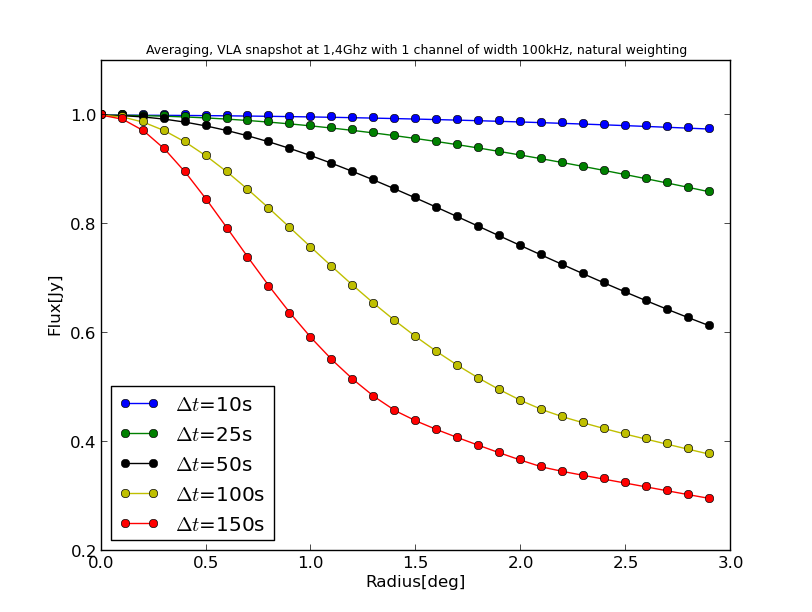
\includegraphics[width=1\textwidth]{./Figures/effect_time_averaging.png}\caption{The fall of the 
intensity of a 1Jy source move from the phase centre for $\Delta t$ integration synthesis at 100KHz 
bandwidth.}\label{timessear1}\end{minipage}
\begin{minipage}{0.38\linewidth}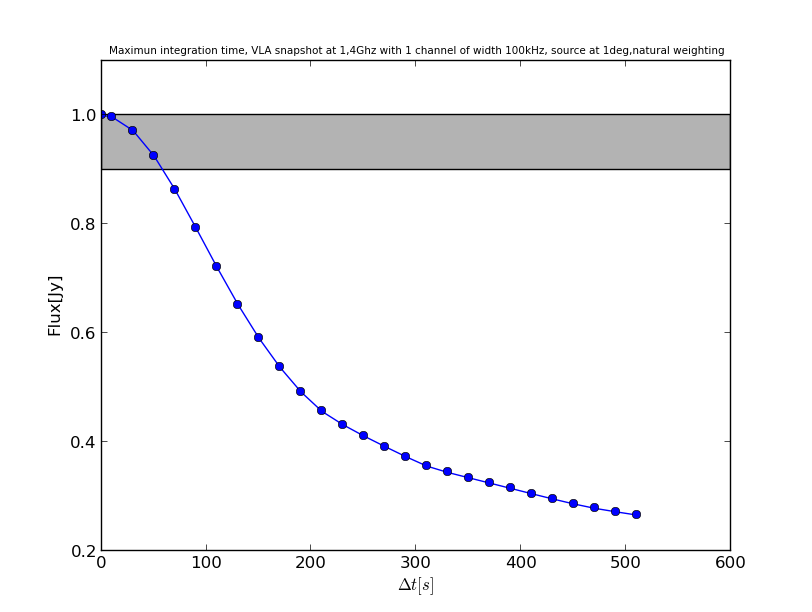
\includegraphics[width=1\textwidth]{./Figures/maximun_integration.png}\caption{(b)Response to a 1Jy 
source at 1deg, as a function of $\Delta t$ with 100KHz bandwidth}\label{timessear11}\end{minipage}\\
\begin{minipage}{0.38\linewidth}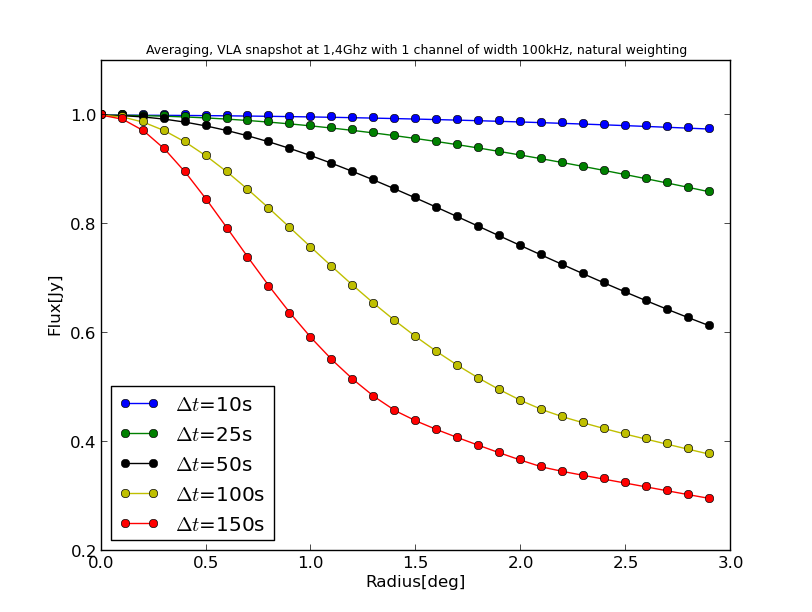
\includegraphics[width=1\textwidth]{./Figures/effect_time_averaging.png}\caption{The fall of the 
intensity of a 1Jy source move from the phase centre for $\Delta t$ integration synthesis at 100KHz 
bandwidth.}\label{timessear2}\end{minipage}
\begin{minipage}{0.38\linewidth}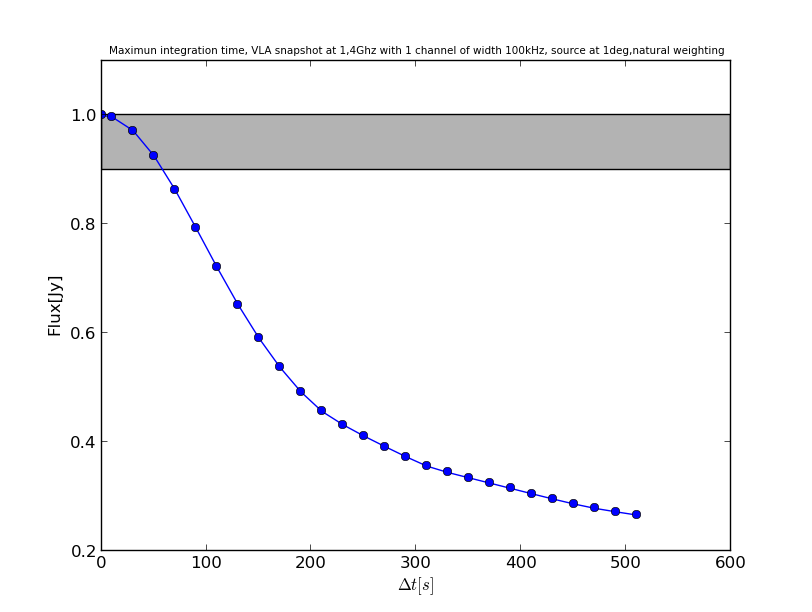
\includegraphics[width=1\textwidth]{./Figures/maximun_integration.png}\caption{The fall of the 
intensity of a 1Jy source move from the phase centre for $\Delta t$ integration synthesis at 100KHz 
bandwidth.}\label{fig:fig_5}\end{minipage}
\end{figure*}
Fortunately, since the response is maximal only for sources at the phase centre, an interesting approach is achieved by convolving the 
observed visibility with a  windowing function that depends on $(u,v)$ coordinates spacing (baseline dependent windowing function).
\subsection{Imaging}
From the full sky Radio Interferometry Measurement Equation (RIME) formalism (see Hamaka et \textit{al}, O.M. Smirnov (2010a)), in this 
case, the sampled visibilities can be presented mathematically as a $4\times n_t\times n_{\nu}$ matrix of four polarizations time and 
frequency dependent matrices each of size $n_t\times n_{\nu}$.
\begin{eqnarray*}
\mathbf{V}_{pq,(t,\nu)}^{samp}&=&\mathcal{\textbf{S}}_{pq,(t,\nu)}\cdot\mathbf{V}_{pq,(t,\nu)}\\
			      &=&\Bigg(\mathbf{V}_{pq,(t,\nu)}^{0},\mathbf { V } 
^1_{pq,(t,\nu)},\mathbf{V}^2_{pq,(t,\nu)},\mathbf{V}_{pq,(t,\nu)}^{3 } \Bigg)^T. \label{eqx:conv}
\end{eqnarray*}
Now, consider that $\mathcal{\textbf{W}}_{pq,(t,\nu)}$ is a $n_t \times n_{\nu}$ matrix that contained the weights of the baseline $(p,q)$ 
visibilities points. The weights of this matrix are given by a baseline dependent windowing function that we described in section 
\ref{baseline1} and section \ref{baseline2}.
The convolution operator is linear, therefore we can rewrite Eq.\ref{f4} in terms of a series of linear transformations as follow:
\begin{equation}
V_{pq}^{avg}= \mathbf{W}_{pq,(t,\nu)}^{block}\cdot 
\mathbf{S}_{pq,(t,\nu)}\cdot\mathbf{V}_{pq,(t,\nu)}.\label{eqbb:linear}
\end{equation}
Here, $\mathbf{W}_{pq,(t,\nu)}^{block}$ is a block diagonal matrix of size $(4n_t n_{\nu})\times(4n_t n_{\nu})$ and the 
block elements are $\mathbf{C}_{pq,(t,\nu)}\cdot\mathcal{\textbf{W}}_{pq,(t,\nu)}$ of size $n_t\times n_{\nu}$, where 
$\mathbf{C}_{pq,(t,\nu)}$ is the centre time interval and centre frequency interval sampling matrix of size $n_t\times n_{\nu}$. This
is the result of the time and frequency integration for the baseline $(p,q)$.

For a synthesis, the baseline $(p,q)$ made a full coverage in the $(u,v)$ plane. Therefore, we can  
package into a single matrix, $\mathbf{V}_{pq,}^{avg}$ of size $(4N_t N_{\nu})\times (4N_t N_{\nu})$ the 
weighted average visibilities of the  baseline $(p,q)$ during the synthesis as follows: 
\begin{equation}
\mathbf{V}_{pq}^{avg}= \mathbf{W}_{pq,(t,\nu)}^{block,n}\cdot\mathbf{S}_{pq,(t,\nu)}^{n}\cdot\mathbf{V}_{pq,(t,\nu)},\label{eq2:block}
\end{equation}
where $N_t$ and  $N_{\nu}$ are the number of time sample and frequency channels entering the Fourier domain. If the synthesis time is $T$ 
and the frequency range is $F$, then $T=N_t \times \Delta t$ and $F=N_{\nu}\times\Delta \nu$. The the size of 
$\mathbf{V}_{pq}^{avg}$ can also be written as $(4N_v^{pq})\times (4N_v^{pq})$, where $N_v^{pq}$ is the 
number of time and frequency visibilities for the baseline $(p,q)$). The matrix $\mathbf{W}_{pq,(t,\nu)}^{block,n}$ is a diagonal block 
matrix of size $(4N_v^{pq}n_t n_{\nu})\times (4N_v^{pq}n_t n_{\nu})$ where each diagonal block is the block diagonal matrix 
$\mathbf{W}_{pq,(t,\nu)}^{block}$ defined above and $n$ is the number of $\mathbf{W}_{pq,(t,\nu)}^{block}$. The sampled visibilities
$\mathcal{\textbf{S}}_{pq,(t,\nu)}^{n}\cdot\mathbf{V}_{pq,(t,\nu)}=\textbf{V}_{pq,(t,\nu)}^{samp,n}$ is a one row matrix of size 
$(N_v^{pq}4 n_t n_{\nu})\times (4 n_t n_{\nu})$ made of $\textbf{V}_{pq,(t,\nu)}^{samp}$ on top of each other. 
\begin{equation}
\mathbf{V}_{pq}^{avg}= \mathbf{W}_{pq,(t,\nu)}^{block,n}\cdot 
\mathbf{S}_{pq,(t,\nu)}^{n}\mathbf{F}\cdot\mathcal{I}_{l,m}^{sky},\label{eqv:linear}
\end{equation}
if the number of pixel in the sky model is $N_{pix}$, then the true sky image vector $\mathcal{I}_{l,m}^{sky}$ has a size of $4N_{pix}$ and 
$\textbf{F}$ is the Fourier transform operator of size $(4N_{pix})\times(4N_{pix})$. 

We are generally interested in using the total set of visibilities over baselines, time and frequencies, having $4\times N_v$ visibilities 
measured over all baselines  and $N_v=n_{bl}\times N_v^{pq}$ in this case. Here, $n_{bl}$ is the number of baseline. We can write
\begin{equation}
 \mathbf{V}_{all}^{avg}=\mathbf{A}\cdot\mathcal{I}_{l,m}^{sky}.
\end{equation}
Here, $\mathbf{A}$ is a matrix of size $(4N_v)\times (4N_{pix})$ made of 
$\mathbf{W}_{pq,(t,\nu)}^{block,n}\cdot\mathcal{S}_{pq,(t,\nu)}^{n}\cdot\mathbf{F}$ on top of each other. The 
dirty image, $\mathcal{I}_{l,m}^{D}$ of size $4N_{pix}$ can then be derived
\begin{equation}
\mathcal{I}_{l,m}^{D}=\mathbf{F}^{H}\cdot\mathbf{A}\cdot\mathcal{I}_{l,m}^{sky}.
\end{equation}
Here, $H$ represents the the conjugate transpose operation also known as a Hermitian transpose and $\mathbf{F}^{H}$ is the inverse 
Fourier transform operator of size $(4N_{pix})\times(4N_{pix})$.
% \begin{figure}
%   \subfloat[]{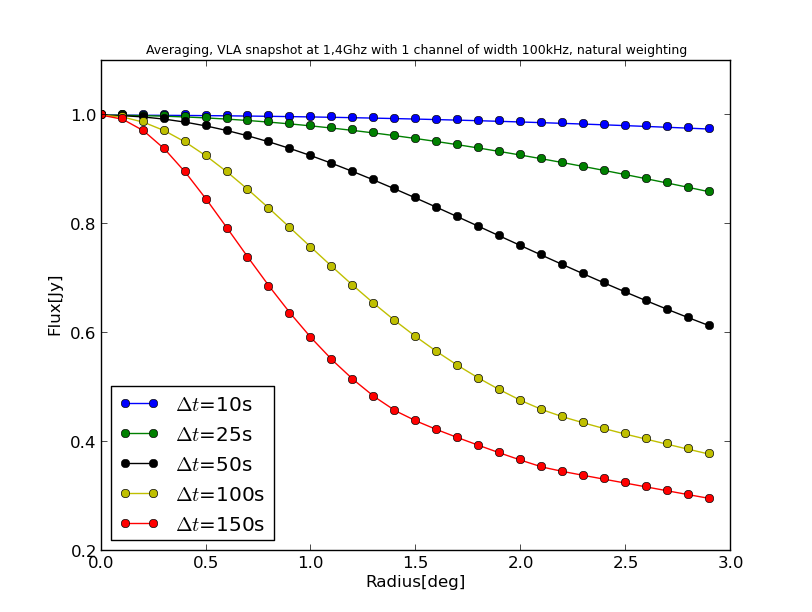
\includegraphics[width=0.18\textwidth, height=0.18\textwidth]{./Figures/effect_time_averaging.png}} 
%   \qquad
%   \subfloat[]{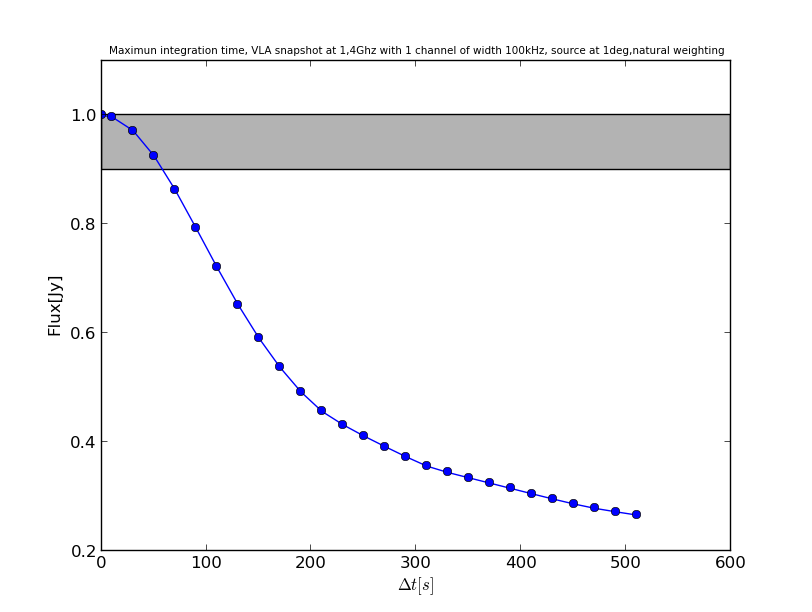
\includegraphics[width=0.18\textwidth,height=0.18\textwidth]{./Figures/maximun_integration.png}}
%   \qquad
%   \subfloat[]{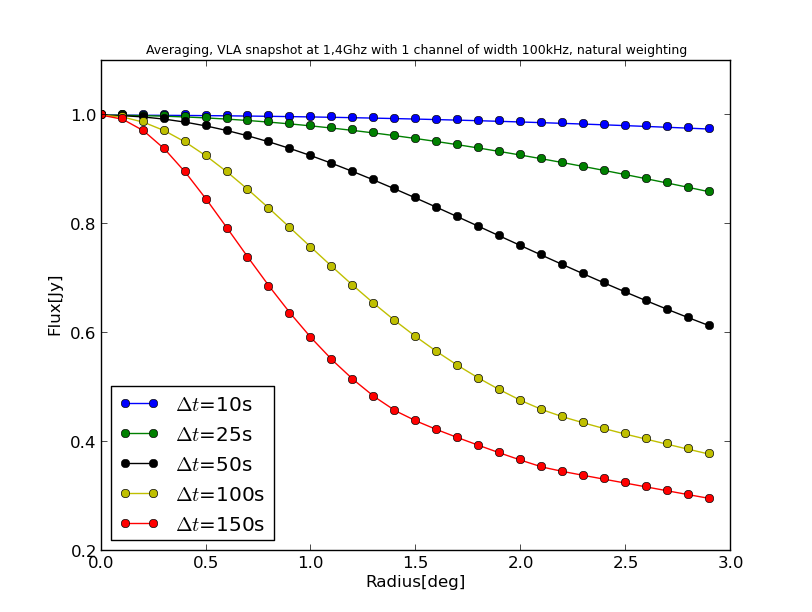
\includegraphics[width=0.18\textwidth, height=0.18\textwidth]{./Figures/effect_time_averaging.png}} 
%   \qquad
%   \subfloat[]{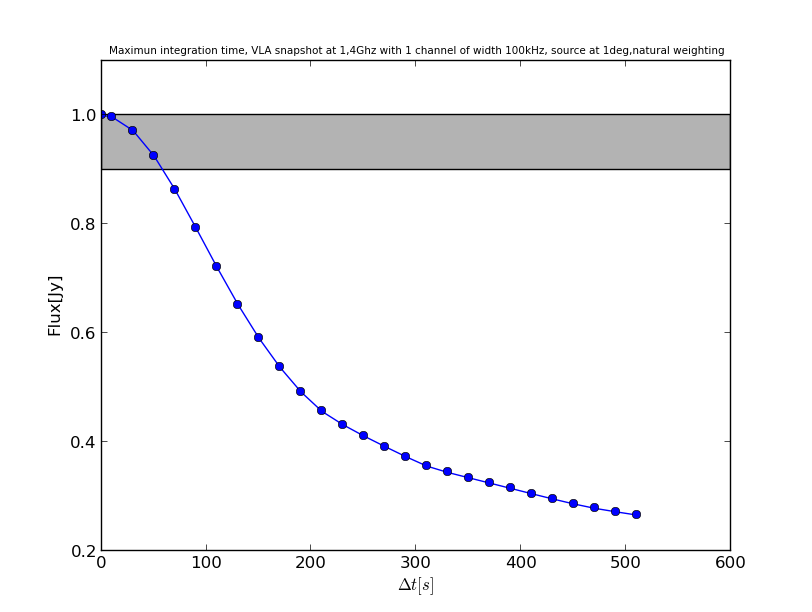
\includegraphics[width=0.18\textwidth,height=0.18\textwidth]{./Figures/maximun_integration.png}}
%   \caption{(a) The fall of the intensity of a 1Jy source move from the phase centre for $\Delta t$ integration synthesis at 100KHz 
% bandwidth. (b)Response to a 1Jy source at 1deg, as a function of $\Delta t$ with 100KHz bandwidth.}
% \end{figure}
\section{Data compression algorithm}
\label{baseline1}
\subsection{Description}
Missing spaces between sampled $(u,v)$ coordinates has huge dependences on the baseline length. However, the spacing between longer 
baselines $(u,v)$ coordinates are wider then the one on shorter baselines: this explained while sources are more distorted on longer 
baselines. We aims in this section, to describe the algorithm we use with a baseline-dependent windowing function to assign a proper 
weight to a data reference by a $(u,v)$ coordinate considering the \textit{spacing}\footnote{The \textit{distance} has also huge 
dependences on the baseline length and allow us to formally define the data
weight of a $uv$ point over the entire $uv$ plane.} between the baseline $(u,v)$ coordinates.

Fig.\ref{fig:uvcov} shows a snapshot coverage of an integration interval. For shorter baselines, the tracks are closer to the centre of 
rotation and for longer baselines the tracks are farther away from this centre. The \textit{dot marks} are the data for a sampled $(u,v)$ 
data, and the  arrows indicates the separation between $(u,v)$ coordinates and the centre $(u,v)$ coordinate. It is trivial to see on this 
figure that these separations are wider on longer baselines. The results of averaging is assigned to the centre $(u,v)$ coordinate coloured 
in red. 
\subsection{Methods}
In this section, we present the data compression algorithm we use to describe the weight of each sampled visibility during the 
integration time interval and and frequency interval. Now, let package the $(u,v)$ coordinates changes of a baseline $pq$ into a single 
matrix of size $n_t \times 2$.
\begin{equation}
\mathbf{U}_{pq,t}= \Bigg(\mathbf{u}_{pq,t_s}, \dots , \mathbf{u}_{pq,t_c}, \dots, \mathbf{u}_{pq,t_e}\Bigg)^T,
\end{equation}
where the indexes $s$, $c$ and $e$ references the integration interval starting, centre, and ending time respectively. The 
elements of $\mathbf{U}_{pq,t}$ are functions of time and frequency representing a $(u,v)$ coordinate. The frequency changes of the 
baseline coordinates can be package into a single vector of dimension $n_{\nu}$ 
\begin{eqnarray*}
 \mbox{\boldmath $\nu$}&=&\Bigg(\nu_s,\dots,\nu_c,\dots,\nu_e\Bigg)^T
\end{eqnarray*}
We define a norm, $||\cdot||_{m}$ on a $n_t \times 2$ matrix as follow:
\begin{eqnarray}
||\textbf{U}_{pq,t}||_{m}=\Bigg(||\mathbf{u}_{pq,t_s}||, \dots , ||\mathbf{u}_{pq,t_c}||, \dots, ||\mathbf{u}_{pq,t_e}||\Bigg),
\end{eqnarray}
where $||.||$ is the Euclidean norm.
\begin{definition}[Time direction spacing]
\label{def:1}
The matrix that model the spacing between the $(u,v)$ coordinates and the centre $(u,v)$ coordinate of a baseline $(p,q)$ across the time 
direction is defined as
\begin{eqnarray*}
 \mathbf{U}_{pq,t}^{s} &=&\frac{\nu_c}{c}\cdot\Bigg\{\mathbf{U}_{pq,t}-\mathbf{H}_{pq,t} \Bigg \},
\end{eqnarray*}
where $c$ is the speed of the light and $\mathbf{H}_{pq}$ is a matrix of size $n_t \times 2$ that model the centre $uv$-coordinate,
$\mathbf{H}_{pq,t}= \big(\mathbf{u}_{pq,t_c}, \dots , \mathbf{u}_{pq,t_c}, \dots, \mathbf{u}_{pq,t_c}\big)^T$.
\end{definition}
\begin{definition}[Frequency direction spacing]
\label{def:2}
The vector of size $n_{\nu}$ that model the spacing between the $(u,v)$ coordinates and the centre $(u,v)$ coordinate of a baseline $(p,q)$ 
across the frequency direction is defined as
\begin{eqnarray*}
\mathbf{d}^{T}_{\nu} &=&\frac{||\textbf{u}_{pq,t_c}||}{c}\cdot\Bigg\{\mbox{\boldmath 
$\nu$}-\nu_c\cdot\mathbf{g}^T_{\nu} \Bigg \},
\end{eqnarray*}
where  $\textbf{g}$ is a $1\times n_{\nu}$ unity matrix.
\end{definition}
\begin{definition}[Baseline dependent windowing function]
\label{def:3}
If $f_{pq}$ is a \textit{baseline dependent windowing function}, then:
\begin{eqnarray*}
 f_{pq}: \{\mathbf{\mathcal{R}},\mathbf{\mathcal{R}}\} &\rightarrow& \mathbf{\mathcal{R}}\\
                   d_{t_i},d_{\nu_j} &\mapsto& \frac{w_{t_i,\nu_j}}{\sum_{i=1}^{n_t}\sum_{j=1}^{n_{\nu}}w_{t_i,\nu_j}}.
\end{eqnarray*}
where $d_{t_i}$ is an element of the vector $\mathbf{d}_{t}=||\mathbf{U}_{pq,t}^{s}||_{m}$ and $d_{\nu_j}$ is an element of the vector 
$\mathbf{d}^{T}_{\nu}$.
\end{definition}
% where $\mathbf{x}_{pq}(t-t_c)=\bigg(\Big|\Big|\Big(u_{pq}'(t_s),v_{pq}'(t_s)\Big)\Big|\Big|,\dots, 
% \Big|\Big|\Big(u_{pq}'(t_e),v_{pq}'(t_e)\Big)\Big|\Big| \bigg)$ and 
% $\mathbf{y}_{pq}(\nu-\nu_c)=\bigg(\Big|\Big|\Big(u_{pq}''(\nu_s),v_{pq}''(\nu_s)\Big)\Big|\Big|,\dots, 
% \Big|\Big|\Big(u_{pq}''(\nu_e),v_{pq}''(\nu_e)\Big)\Big|\Big| \bigg)  $
% $1.)$ In Figures (\ref{fig1}) and (\ref{fig2}) we represented the ratio $\frac{\sigma_{meas,pq}}{\sigma_{av,pq}}$ as a function 
% of $\sum_{i}^{n} u_i((t_c-t_i)/\lambda))$ ($\sigma_{meas,pq},\sigma_{av,pq}$ are the per baselines CWF and averaging rms noise  
% respectively). We could also represented it as a function of baseline length. But, a uv-track corresponding to baseline aligned along the 
% Est-West direction has longer tracts compare to one aligned along the South-Nordth for the same integration and frequency band. Therefore,  
% $\frac{\sigma_{meas,pq}}{\sigma_{av,pq}}$ $v/s$ baselines length is ambiguous. We consider five baselines dependent 
% windowing sinc function, $Bl$-$sinc$ $wk$ (with an extended width of $(k-1)n$ time intervals and/or frequency channels and $k \geq 1$). The 
% experiment is done for two cases, figure (\ref{fig1}) is the one for $Bl$-$sinc$ $wk$ over both time-frequency and figure (\ref{fig2}) over 
% time. These figures shows that, the noise increases with baselines length.\\
% \begin{figure}
%   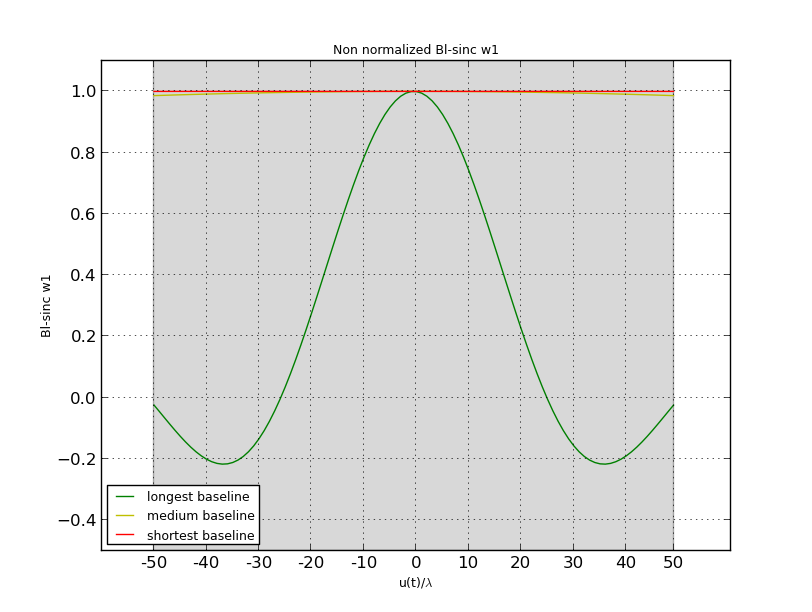
\includegraphics[width=0.4\textwidth, height=0.4\textwidth]{./Figures/longshortmid.png}
%   \caption{Snapshot coverage} \label{uvcov}
% \end{figure}
% \begin{figure}
%   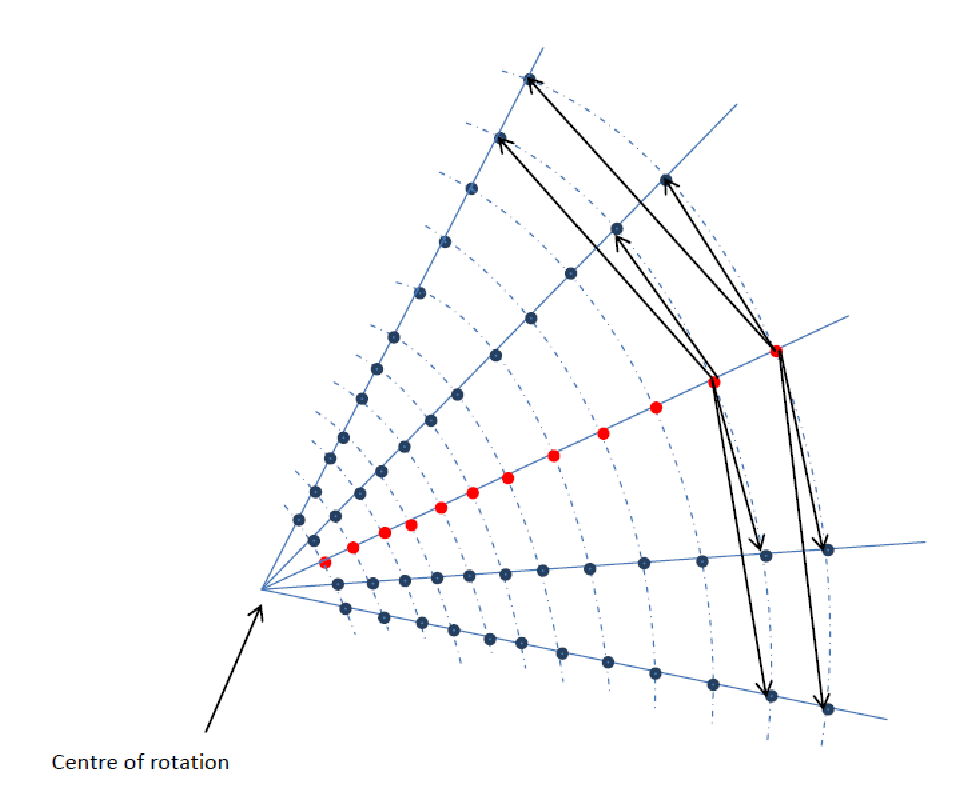
\includegraphics[width=0.4\textwidth, height=0.4\textwidth]{./Figures/uvcov.png}
%   \caption{Snapshot coverage} \label{uvcov}
% \end{figure}
\begin{figure*}
 \centering
\begin{minipage}{0.38\linewidth}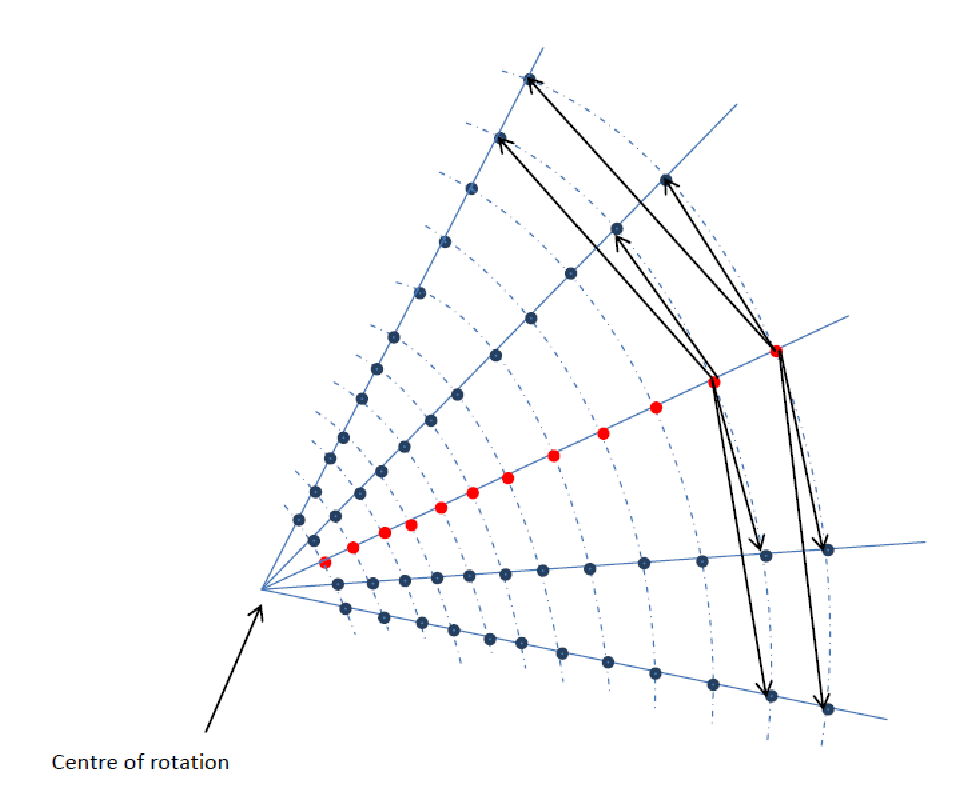
\includegraphics[width=1\textwidth]{./Figures/uvcov.png}\caption{Snapshot coverage}\label{fig:uvcov} 
\end{minipage}
\begin{minipage}{0.38\linewidth}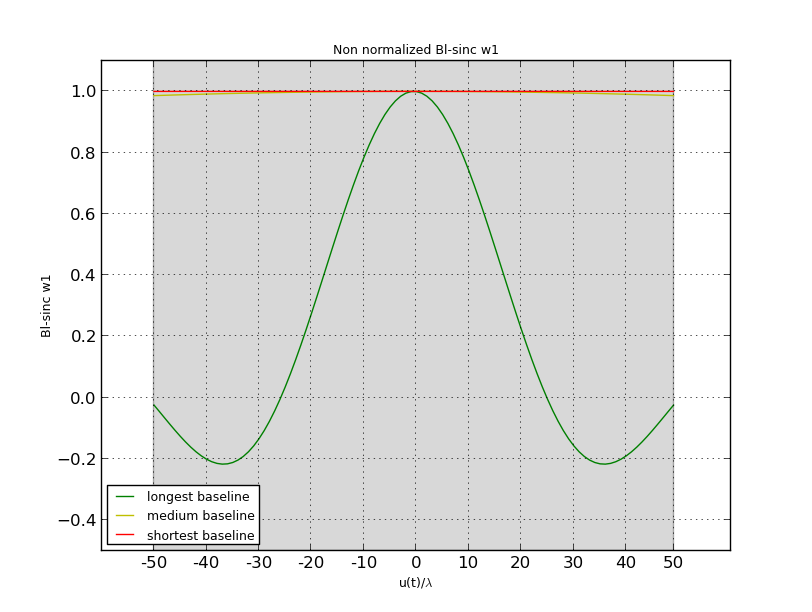
\includegraphics[width=1\textwidth]{./Figures/longshortmid.png}\caption{$Bl$-$sinc w1$ used to convolve the 
visibility data obtained from the long, medium and short baseline}\label{fig:fig_2b}
\end{minipage}
\end{figure*}
% \subsection{Cross-correlation with \textit{BDWF}}
% Taking a step back to eq \ref{}
% \begin{eqnarray*}
%  V^{meas}_{pq}(\mathbf{u}(t)/\lambda) &=&\sum_{t}\sum_{\nu} f_{pq}(\mathbf{d}_{t},\mathbf{d}_{\nu})\cdot 
% \mathbf{V}_{pq}^{obs}(t,\nu)\\
% 					  &=& \sum_{t}\sum_{\nu}\mathbf{W}_{pq}(t-t_c, \nu-\nu_c)\cdot \mathbf{V}_{pq}^{obs}(t,\nu)\\
% \end{eqnarray*}
\subsection{Noise  analysis}
% In this section, theoretical expressions of the noise of correlator windowing functions (CWF) are derived. 
% Simulations results shows that when the overlap width of CWF is increased, the noise in the sky map is reduced. Furthermore, 
% the noise reduces more rapidly when the overlap is done over both time intervals and frequency channels. For convenience, we have 
% chosen to derive the analytical expression for the noise of a CWF at the phase centre. For the analysis we used a simulated 
% VLA, 1min30s synthesis, with a 1,5s integration time at 1,4Ghz, with 100 channels of width 1kHz. We fill this simulated measurement set 
% with 1Jy thermal noise and we used a sinc as a CWF.
For convenience, in this section, we  analyse the centre pixel noise of a sky map after we had apply a baseline dependent windowing 
function during the time and frequency integration. The brightness of the 
naturally weighted central pixel is estimate by (see the inverse Fourier transform of equation (19-2) in 
\cite{1} ).
\begin{eqnarray*}
\widetilde{\mathcal{I}}(0,0)&=&\frac{1}{N_{v}}   \sum_{k=1}^{N_{v}} V_{all,k}^{avg}\\
	          &=&\frac{1}{N_{v}}   \sum_{pq,k=1}^{N_{v}^{pq}} V_{pq,k}^{avg}\\
	          &=&\frac{1}{N_{v}}   \sum_{pq,k=1}^{N_{v}^{pq}}\Big(\sum_{i=1}^{n_t}\sum_{j=1}^{n_{\nu}} 
f_{pq,(dt_i,d\nu_j)}V_{pq,(t_i,\nu_j)}^{samp}\Big).
\end{eqnarray*}
Here, the variable $k$ run through the baseline $(p,q)$ timeslots. The  overall rms noise is given by
\begin{eqnarray*}
\sigma^2	&=& 
\frac{\sigma^{2}_{samp} }{N_{v}^{2}}\Big(\sum_{pq,k=1}^{N_{v}^{pq}}\sum_{i=1}^{n_t}\sum_{j=1}^{n_{\nu}}f_{pq,(dt_i,d\nu_j)}^{2}\Big) ,
\end{eqnarray*}
where  $\sigma_{samp}$ is the per sampled visibility noise
% Where $W^{pq}$ is a normalized CWF; $\lambda$, $t_c$ are the observed wavelength and centre of the integration 
% respectively. $N_{meas}$ is the number of the measured visibilities. The observed visibilities of baseline $pq$  are 
% $V^{pq}_{obs}(u(t/\lambda))$, $n$ is the number of time intervals  and/or frequency channels within the within the width of the CWF.
% %and defined as % and is given by
% let introduced jjjjjjjjjjjjjjs  sjjs lkk xxxxxxxxxxxx xxxxxxxxxxxx xxxxxxxxxx xxxxxxxxxx xxx ,xssss, s,,,sssssx, xxxxxxxxxx,x 
% xxxxxxxxxxxxxx,,xxxxxxxxxxxx, write more here to explain
% \begin{eqnarray**}
% \widetilde{I}(0,0)&=&\frac{1}{N_{meas}}   \sum_{all-pq}\Big(\sum_{t}\sum_{\nu}f_{pq}(\mathbf{d}_{t},\mathbf{d}_{\nu})\cdot 
% \mathbf{V}_{pq}^{obs}(t,\nu)\Big)
% \end{eqnarray**}
% \begin{eqnarray*}
% 		\sigma_{meas, pq}^2	&=&var\Big(\sum_{t}\sum_{\nu}f_{pq}(\mathbf{d}_{t},\mathbf{d}_{\nu})\cdot 
% \mathbf{V}_{pq}^{obs}(t,\nu)   
% \Big)\\
% 		&=&\sum_{t}\sum_{\nu}f_{pq}^{2}(\mathbf{d}_{t},\mathbf{d}_{\nu}) \sigma_{obs}^2 
% \end{eqnarray*}
% where $\sigma_{obs}$ is the expected rms noise per observed visibility. By replacing eq \ref{1} into eq \ref{1} we obtained
% \begin{eqnarray*}		
% \sigma^2	
% &=&\Big(\frac{\sigma_{obs}}{N_{meas}}\Big)^2\cdot\sum_{all-pq}\Big(\sum_{t}\sum_{\nu}f_{pq}^{2}(\mathbf{d}_{t},\mathbf{d}_{\nu})\Big)
% \end{eqnarray*}
% If $f_{pq}$ is a boxcar function, then $\sigma^2 =\frac{1}{N_{meas} \times n_t \times n_{\nu}} \sigma_{obs}^2$ ,
% and can be expressed as a function of the number of the observed visibilities, $N_{obs}$ as $\sigma^2=\frac{1}{N_{obs}\times 
% n_{\nu}} \sigma_{obs}^2$.
% % \begin{eqnarray**}
% % \sigma^2	   &=&\frac{1}{N_{obs}\times n_{\nu}} \sigma_{obs}^2
% % \end{eqnarray**}
\section{Out FoV sources suppression algorithm}
\label{baseline2}
\subsection{Description}
In theory, windowing functions and signals generally extend to  infinity. Unfortunately, in practice, filtering a signal with a low pass 
filter, one need to define a cut-off interval. Therefore, if one  wants to achieve sufficiently an accurate  estimate of the 
windowing function ideal spectrum, one need a wide cut-off interval as far as the spectrum approaches the ideal when the windowing function 
order increases. An overlap baseline dependent windowing function aims to extend the order of the baseline dependent windowing function in 
such a way that, we approaches the ideal spectrum.
%, but by maintaining the same cut-off interval like the boxcar one. 
The only drawback of this technique is the increased of the time needed for processing the output sample of the signals being integrate.  
\subsection{Methods}
The weight of a visibility is not defined by a unique baseline dependent windowing, but by the strength of the correlation between the 
overall  overlapping baseline dependent windowing functions on the visibility. Now, consider that $f^{a}_{pq}$ is an overlap-\textit{BDWF} 
of width  $\Delta t$ and $\Delta \nu$ across the time and frequency direction respectively.
\begin{definition}[Baseline dependent windowing function]
\label{def:4}
if $\Delta_l t$ and $\Delta_l \nu$ are the overlap time interval and frequency interval of the baseline dependent windowing function  
$f_{pq}^{a_0}$ respectively  and $\Big\{f_{pq}^{a_1},f_{pq}^{a_2},f_{pq}^{a_3}, \dots \Big\}$ the set of \textit{BDWF} overlapping  on the 
\textit{left hand side} of $f_{pq}^{a_0}$ then the resulting \textit{BDWF} within $\Delta_l t$ and $\Delta_l \nu$ is defined as
\begin{eqnarray*}
 g^{lhs}_{pq}: \{\mathbf{\mathcal{R}},\mathbf{\mathcal{R}}\} &\rightarrow& \mathbf{\mathcal{R}}\\
                   d_{t_i},d_{\nu_j} &\mapsto& \frac{1}{N_{lhs}}\Bigg(\sum_{k}f_{pq,(d_{t_i},d_{\nu_j})}^{a_k} 
+ f_{pq,(d_{t_i},d_{\nu_j})}^{a_0}\Bigg).
\end{eqnarray*}
Here, $N_{lhs}$ is the normalization term defined as
\begin{eqnarray*}
N_{lhs}=\sum_{i=1}^{n_{lt}}\sum_{j=1}^{n_{l\nu}}\Bigg(\sum_{k}f_{pq,(d_{t_i},d_{\nu_j})}^{a_k} + f_{pq,(d_{t_i},d_{\nu_j})}^{a_0} \Bigg),
\end{eqnarray*}
where $n_{lt}$ and $n_{l\nu}$ are the number of $(u,v)$ coordinates changes and frequency changes  within $\Delta_l t$ and $\Delta_l \nu$ 
respectively.
\end{definition}
\begin{definition}[Baseline dependent windowing function]
 \label{def:4}
 if $\Delta_r t$ and $\Delta_r \nu$ are the overlap time and frequency interval of a \textit{BDWF} $f_{pq}^{a_0}$ 
respectively and  $\Big\{f_{pq}^{a_1},f_{pq}^{a_2},f_{pq}^{a_3}, \dots \Big\}$ the set of \textit{BDWF} overlapping on the \textit{right 
hand side} of $f_{pq}^{a_0}$, then the 
resulting \textit{BDWF} within $\Delta_r t$ and $\Delta_r \nu$ is defined as
\begin{eqnarray*}
 g^{rhs}_{pq}: \{\mathbf{\mathcal{R}},\mathbf{\mathcal{R}}\} &\rightarrow& \mathbf{\mathcal{R}}\\
                   d_{t_i},d_{\nu_j} &\mapsto& 
\frac{1}{N_{rhs}}\Bigg (f_{pq,(d_{t_i},d_{\nu_j})}^{a_0}+\sum_{k}f_{pq,(d_{t_i},d_{\nu_j})}^{a_k}\Bigg ).
\end{eqnarray*}
Here, $N_{rhs}$ is the normalization term defined as
\begin{eqnarray*}
N_{rhs}=\sum_{i=1}^{n_{rt}}\sum_{j=1}^{n_{r\nu}}\Bigg(f_{pq,(d_{t_i},d_{\nu_j})}^{a_0} + \sum_{k}f_{pq,(d_{t_i},d_{\nu_j})}^{a_k}\Bigg),
\end{eqnarray*}
where $n_{rt}$ and $n_{r\nu}$ are the number of $(u,v)$ coordinates changes and frequency changes  within $\Delta_r t$ and $\Delta_r \nu$ 
respectively.
\end{definition}
From the above definitions, the following derivation is trivial 
\begin{equation*}
 \Big\{\Delta t,\hspace{0.17cm}\Delta \nu \Big\}=\Big\{\Delta_l t \cup \Delta_u t \cup \Delta_r t, \hspace{0.17cm}\Delta_l \nu \cup 
\Delta_u \nu \cup \Delta_r \nu \Big\},
\end{equation*}
where $\Delta_u t$ and $\Delta_u \nu$ are $f_{pq}^{a_0}$ uncorrelated time  and frequency interval respectively. They follows the below 
rules 
\begin{eqnarray*}
 \Delta_u t= \left\{ 
  \begin{array}{l l}
     \cup\{t_i\}_{i=s',\hspace{0.1cm} s' \geq s+1}^{c', \hspace{0.1cm}c'\leq c-1} & \quad \text{if $n_{lt}+n_{rt}< n_t$}\\
      \{t_c\}& \quad \text{if $n_{lt}+n_{rt} = n_t$}\\
       \emptyset  & \quad \text{otherwise}
  \end{array} \right.
\end{eqnarray*}
\begin{eqnarray*}
 \Delta_u \nu= \left\{ 
  \begin{array}{l l}
     \cup\{\nu_i\}_{i=s',\hspace{0.1cm} s'\geq s+1}^{c', \hspace{0.1cm}c'\leq c-1} & \quad \text{if $n_{lt}+n_{rt} < n_t$}\\
      \{\nu_c\}& \quad \text{if $n_{lt}+n_{rt} = n_t$}\\
       \emptyset  & \quad \text{otherwise}
  \end{array} \right.
\end{eqnarray*}
The resulting \textit{BDWF} becomes $g_{pq}$ described as
\begin{eqnarray*}
g_{pq} = \left\{ 
  \begin{array}{l l}
    g^{lhs}_{pq} & \quad \text{if $(t,\nu) \in (\Delta_l t, \Delta_l \nu)$}\\
    f^{a_0}_{pq} & \quad \text{if $(t,\nu) \in (\Delta_u t, \Delta_u \nu)$}\\
    g^{rhs}_{pq}& \quad \text{if $(t,\nu) \in (\Delta_r t, \Delta_r \nu)$}
  \end{array} \right.
\end{eqnarray*}
\subsection{Noise analysis}
The  overall rms noise is given by
\begin{eqnarray*}
\sigma^2	&=& 
\frac{\sigma^{2}_{samp} }{N_{v}^{2}}\Big(\sum_{pq,k=1}^{N_{v}^{pq}}\sum_{i=1}^{n_t}\sum_{j=1}^{n_{\nu}}g_{pq,(dt_i,d\nu_j)}^{2}\Big) ,
\end{eqnarray*}
\subsection{Weighting functions}
In signal processing a windowing function is a mathematical function that is zero-values outside of some chosen interval, and when another 
function or a signal is multiplied by the windowing function, the product is also zero-values outside the interval.
In this section, we evaluation the Peak Sidelobe Level, the Main 
Lobe width and the Sidelobes Roll-of of the spectrum of some windowing functions. This study will allow us to make 
a suitable choice of the window that by tapering with the sky, we conserve the brightness of sources in the field of interest and  
attenuate sidelobes confusion from strong sources out of the field of interest.
\subsubsection{Boxcar window: natural weighting}
This windowing function take a hunk of the data without modification, and  this leads to discontinuities at the edges\footnote{unless it 
happens that the signal  fit exactly with the windowing function width. Nevertheless, it is rare to find such a situation.}. For 
a cut-of frequency interval  $[-\nu_e/2,\nu_e/2]$ the boxcar windowing function is defined as:
\begin{equation}
\Pi_{u}=\left\{
\begin{array}{rl}
1 & \mbox{$-\nu_a/2 \leq \nu \leq \nu_a/2$} \\
0 & \mbox{otherwise}
\end{array}\right.
\end{equation}
and it Fourier transform is $\mathcal{F}^{-1}\big\{\Pi_{u}\big\}=sinc\big(\pi ||u(t/\lambda_a)|| l\big)$.\\
Fig.\ref{fig:box} gives the graph of $\mathcal{F}^{-1}\big\{\Pi_{u}\big\}$. The main lobe extends from $-1/(2\nu_a)$ to $1/(2\nu_a)$, 
beyond that the function oscillates at a constant rate while the amplitude gradually dies out. The larger the $\nu_a$, the narrower the 
central peak and the oscillations.
\subsubsection{Gaussian window}
A Gaussian windowing function centred at mean zero with standard deviation, $\sigma$ can be described as 
\begin{equation}
  G_{u}= e^{-b||u(t/\lambda_a)||^{2}},
\end{equation}
where $b=(2\sigma^2)^{-1}$ and  $\mathcal{F}^{-1}\big\{G_{u}\big\}=\sqrt{\frac{b}{\pi}}e^{-cl^2}$, where $c=\pi^2/b$
This shows us that the inverse Fourier transform of a Gaussian with standard deviation $\sigma$ is a Gaussian with a standard 
deviation $\sigma '= (2\pi\sigma)^{-1}$ . In theory, the Gaussian window is an infinitely large convolution filter as it is non zero 
everywhere. However, in practice some one need to defined a cut-off interval where the window is considered to be non zero, and zero out of 
this cut-off interval. 
Fig.\ref{fig:Gauss} and \ref{fig:GaussFou} gives the graph of $G_{u}$ and $\mathcal{F}^{-1}\big\{G_{u}\big\}$, where $G_{u}$ is truncate 
within the cut-off frequency interval $[-\nu_e/2,\nu_e/2]$, with $\sigma =1$. The main lobe of $\mathcal{F}^{-1}\big\{G_{u}\big\}$ extends 
from $-(2\pi\sigma)^{-1}$ to $(2\pi\sigma)^{-1}$, beyond that the amplitude gradually dies out. The larger the $\sigma$, the narrower the 
central peak.
\subsubsection{Butterworth}
The frequency response of the Butterworth filter is flat  in the pass band, and rolls off towards zero in the stop band, and it is 
characterized by two independent parameters, the cut-off frequency 
$\nu_a$ and the order $p$. These two parameters controls the 
bandwidth and side lobes  attenuation. The frequency response of the Butterworth is given by 
\begin{equation}
B_u= \Big(1 + (||u(t/\lambda_a)||/\nu_a)^{2p}\Big)^{-1}
\end{equation}
Fig.\ref{fig:buter} gives the graph of $B_{u}$. The inverse  Fourier transform is applied to $B_{u}$, in Fig.\ref{fig:buterFou}. The main 
lobe of 
$\mathcal{F}^{-1}\big\{B_{u}\big\}$ extends from $-(2\pi\sigma)^{-1}$ to $(2\pi\sigma)^{-1}$, beyond that the amplitude gradually dies out. 
The larger the $\sigma$, the narrower the central peak.
\subsubsection{First order prolate spheroidal wave function}


A windowing function with a narrower main lobe width and a smaller ripple is preferably in this application. Nevertheless, when the 
frequency domain main lobe width is small, the energy is concentrated in that array. The result of the 
rectangular window and the Butterworth window look similar but, we can adjust the Butterworth window as we want by manipulating the 
parameter $p$ to concentrate more energy in the frequency main lobe.
\subsubsection{Noise performance analysis and comparison}
The methods described in section (\ref{baseline1}) and section (\ref{baseline2}) are use in this subsection to evaluate the 
theoretical noise of each of the above windowing functions. Table (\ref{BDWBnoise}) summarize the theoretical noise of the above windowing 
function used as a baseline dependent windowing, and table (\ref{OBDWBnoise}) is the theoretical noise of the above windowing 
function used as an overlap baseline dependent windowing functions.\\
\begin{tabular}{*3{c}}
 \multicolumn{3}{c}{}\\
  \hspace{-1.cm}\begin{tabular}{|c|c|}
  \textbf{$f_{pq}$}&\textbf{\footnotesize Theoretical noise} \\
  \hline\hline
  {\footnotesize $\Pi_{u}$} &{\footnotesize 1,066} \\ 
  {\footnotesize $\mathcal{F}^{-1}\{\Pi_{u}$\}} &{\footnotesize 1,066} \\
  {\footnotesize $G_{u}$} & {\footnotesize 1,334}\\ 
  {\footnotesize $B_{u}$} &{\footnotesize 1,066} \\
  {\footnotesize $\mathcal{F}^{-1}\{B_{u}$\}} &{\footnotesize 1,066} \\ 
  {\footnotesize $P_{u}$} & {\footnotesize 1,334}
  \end{tabular}& \label{BDWBnoise}
   \begin{tabular}{|c|c|}
  \textbf{$g_{pq}$}&\textbf{\footnotesize Theoretical noise} \\
  \hline\hline
  {\footnotesize $\Pi_{u}$} &{\footnotesize 1,066} \\ 
  {\footnotesize $\mathcal{F}^{-1}\{\Pi_{u}\}$} &{\footnotesize 1,066} \\
  {\footnotesize $G_{u}$} & {\footnotesize 1,334}\\ 
  {\footnotesize $B_{u}$} &{\footnotesize 1,066} \\
  {\footnotesize $\mathcal{F}^{-1}\{B_{u}$\}} &{\footnotesize 1,066} \\ 
  {\footnotesize $P_{u}$} & {\footnotesize 1,334}
  \end{tabular} \label{OBDWBnoise}
\end{tabular}
\\
\\
\\
\begin{figure*}
  \centering
  \begin{minipage}{0.38\linewidth}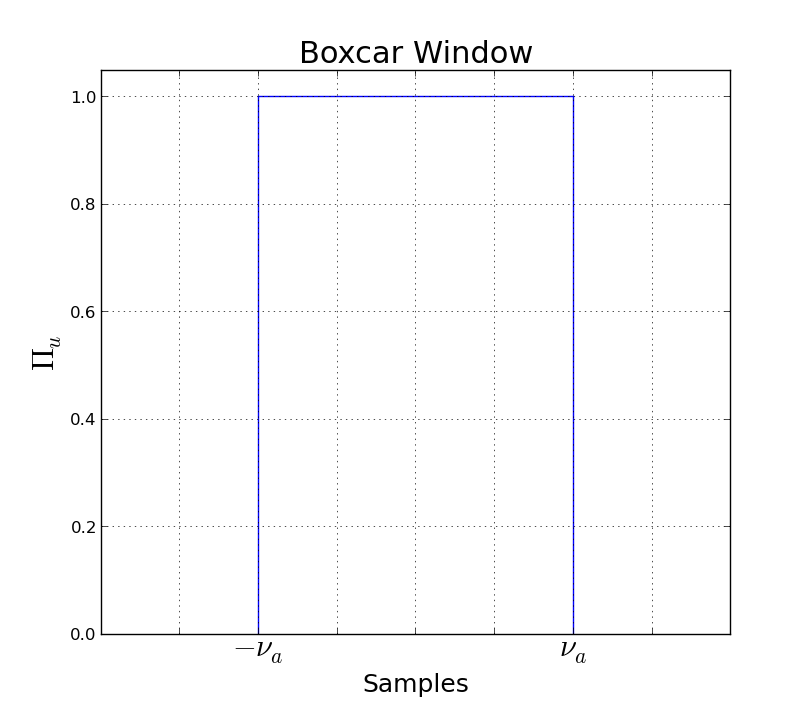
\includegraphics[width=1\textwidth]{./Figures/rect.png}\caption{Overlap 
		\textit{BDWF's}: $\Delta_u t= [225, 250]$.}\label{ fig:fig_3a}\end{minipage}
\begin{minipage}{0.38\linewidth}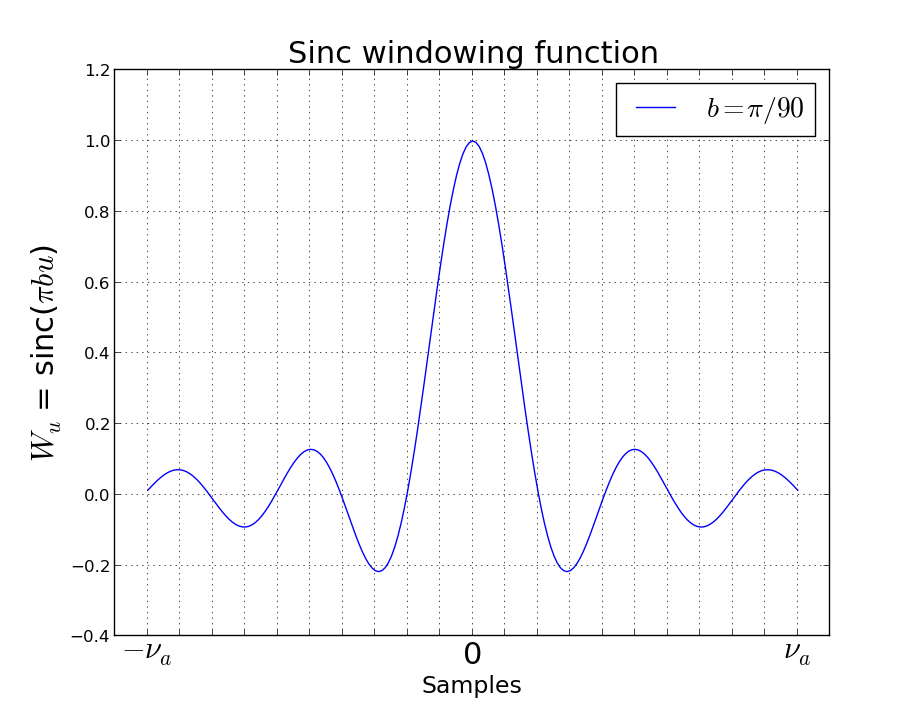
\includegraphics[width=1\textwidth]{./Figures/sinc.png}\caption{Overlap 
		\textit{BDWF's}: $\Delta_u t= [225, 250]$.}\label{ fig:fig_3a}\end{minipage}\\
\begin{minipage}{0.38\linewidth}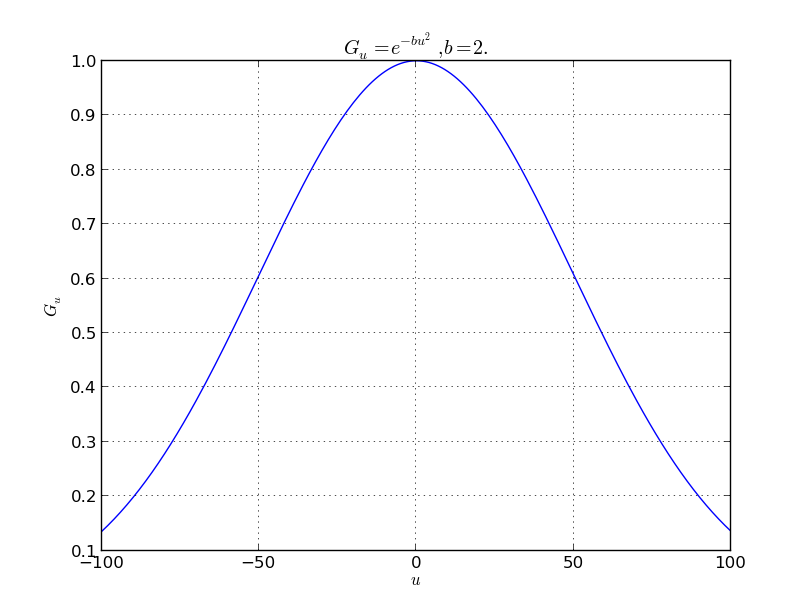
\includegraphics[width=1\textwidth]{./Figures/gausian.png}\caption{Overlap 
		\textit{BDWF's}: $\Delta_u t=\{250\}$.}\label{fig:fig_4}\end{minipage}
\begin{minipage}{0.38\linewidth}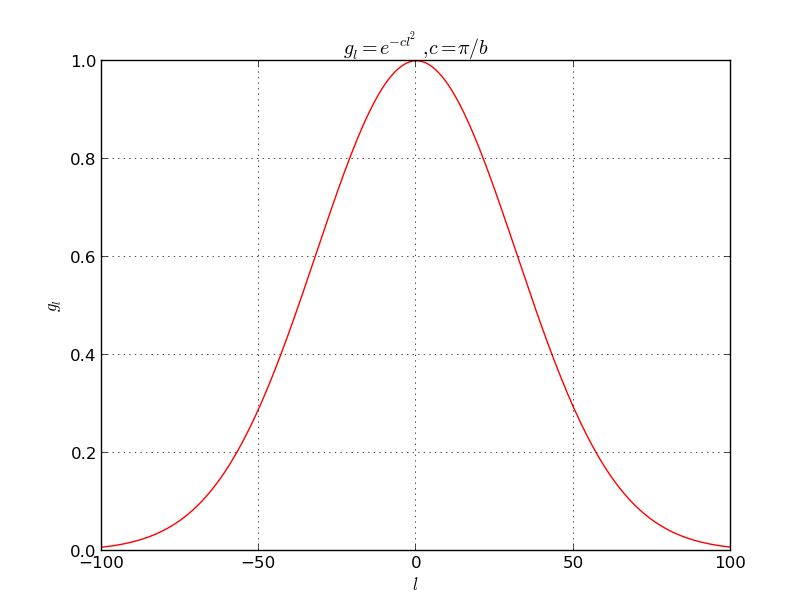
\includegraphics[width=1\textwidth]{./Figures/gausianFour.png}\caption{Overlap 
		\textit{BDWF's}: $\Delta_u t=\emptyset$.}\label{fig:fig_5}\end{minipage}\\
\begin{minipage}{0.38\linewidth}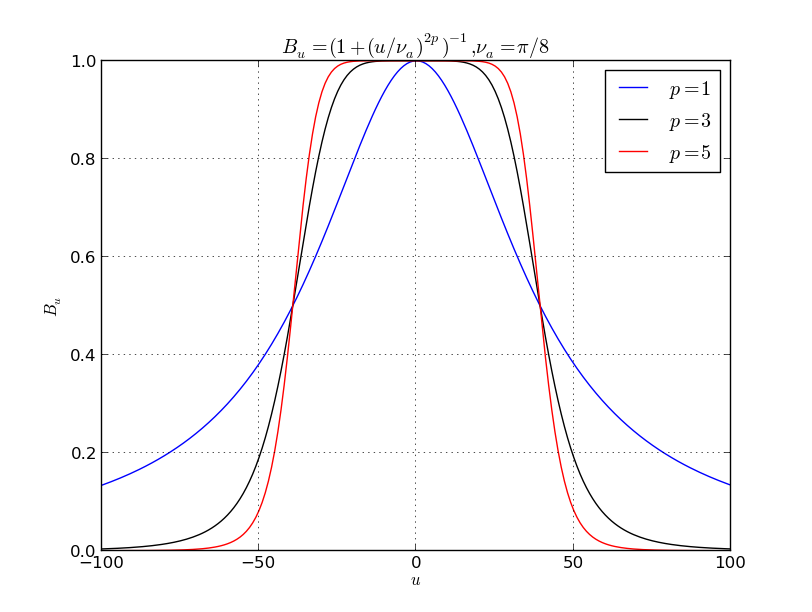
\includegraphics[width=1\textwidth]{./Figures/Butterwordth.png}\caption{Overlap 
		\textit{BDWF's}: $\Delta_u t=\{250\}$.}\label{fig:fig_4}\end{minipage}
\begin{minipage}{0.38\linewidth}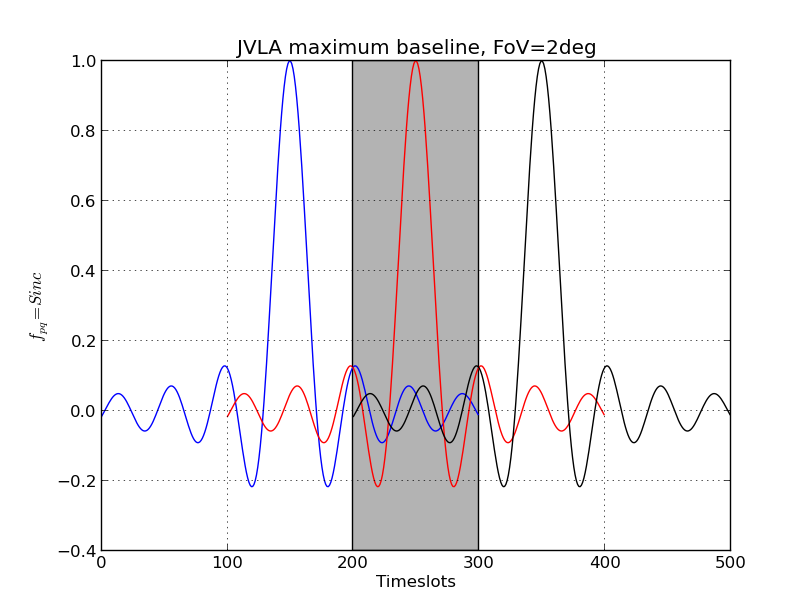
\includegraphics[width=1\textwidth]{./Figures/corrSigVLAMxBl_overlapGdelta.png}\caption{Overlap 
		\textit{BDWF's}: $\Delta_u t=\emptyset$.}\label{fig:fig_5}\end{minipage}\\
\begin{minipage}{0.38\linewidth}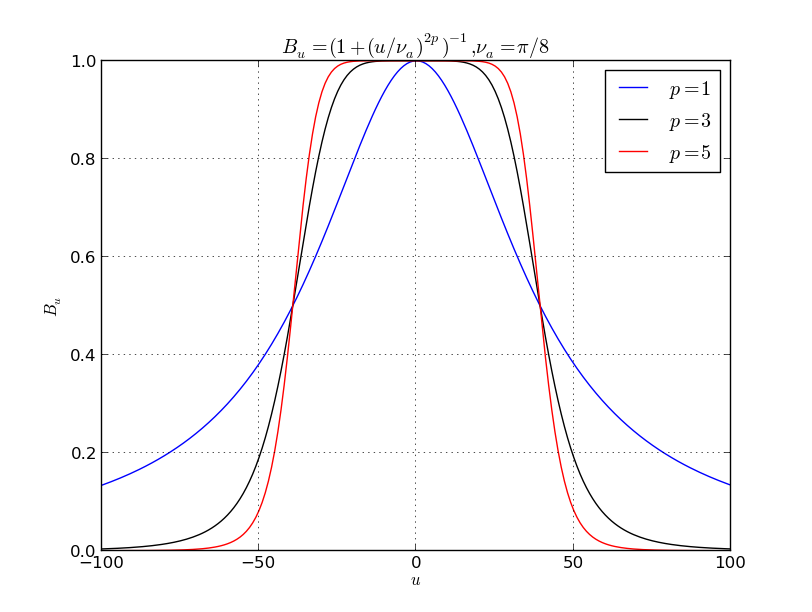
\includegraphics[width=1\textwidth]{./Figures/Butterwordth.png}\caption{Overlap 
		\textit{BDWF's}: $\Delta_u t=\{250\}$.}\label{fig:fig_4}\end{minipage}
\begin{minipage}{0.38\linewidth}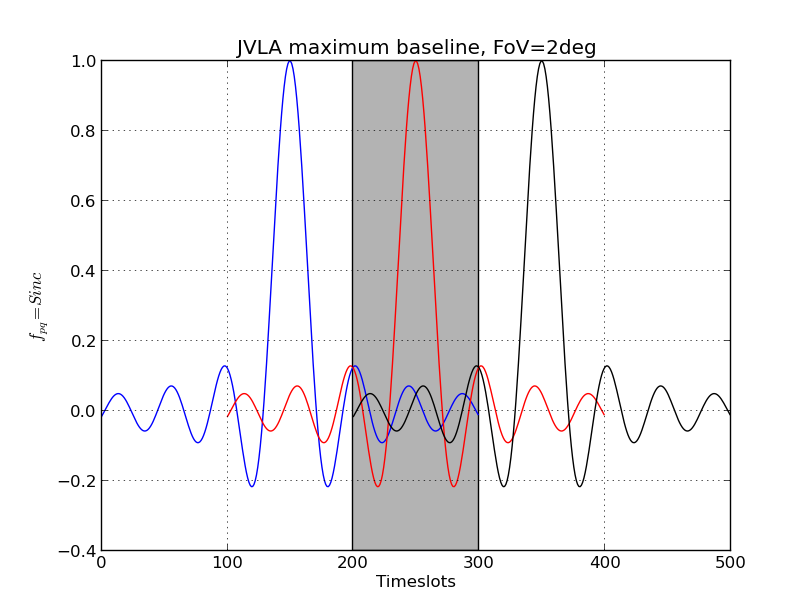
\includegraphics[width=1\textwidth]{./Figures/corrSigVLAMxBl_overlapGdelta.png}\caption{Overlap 
		\textit{BDWF's}: $\Delta_u t=\emptyset$.}\label{fig:fig_5}\end{minipage}\
\end{figure*}

$1.)$ In Figure
% The specification of the weight of the point $(u_k, v_k)$ is, $w(u_k, v_k)=e^{(\frac{-d}{s})^2}$, where $s$ measure the width 
% of the taper and $d=(u_k^2 + v_k^2)^{\frac{1}{2}}$ the baseline length.  However, the rms noise of the central pixel map is given by 
% $\sigma^2=\frac{\sum w^2(u_k, v_k)}{(\sum w^2(u_k, v_k))^2}\sigma_{obs}^2$ (see \cite{}).
% \begin{enumerate}
%  \item (Fig1a) shows the reduction of the intensity of a source at various coordinates in the sky for different $\Delta t$ with 
%        the VLA array. We measured  more than $90\%$ of the source brightness for $\Delta t \leq 25s$ when the source is within the 
%        Field of view. But, we should have compromised the large amount of data generated with shorter $\Delta t$ if the source intensity 
%        should have been drop significantly out of the field of view. For a source at coordinates (l=0, m=1deg) smearing occurs for an 
%        integration greater than 90s (see Fig1b)
%   \item (Fig1c) shows the reduction of the intensity of a source at various coordinates in the sky for different $\Delta t$ with 
%        the VLA array. We measured  more than $90\%$ of the source brightness for $\Delta t \leq 25s$ when the source is within the 
%        Field of view. But, we should have compromised the large amount of data generated with shorter $\Delta t$ if the source intensity 
%        should have been drop significantly out of the field of view. For a source at coordinates (l=0, m=1deg) smearing occurs for an 
%        integration greater than 90s (see Fig1b)
% \end{enumerate}
% \begin{enumerate}
%  \item Fig \ref{fig:fig_3a} shows three \textit{BDWF} design with a $sinc$ filter across the time direction.  
%   \item (Fig1c) shows the reduction of the intensity of a source at various coordinates in the sky for different $\Delta t$ with 
%        the VLA array. We measured  more than $90\%$ of the source brightness for $\Delta t \leq 25s$ when the source is within the 
%        Field of view. But, we should have compromised the large amount of data generated with shorter $\Delta t$ if the source intensity 
%        should have been drop significantly out of the field of view. For a source at coordinates (l=0, m=1deg) smearing occurs for an 
%        integration greater than 90s (see Fig1b)
% \end{enumerate}
\begin{figure*}
  \centering
  \begin{minipage}{0.38\linewidth}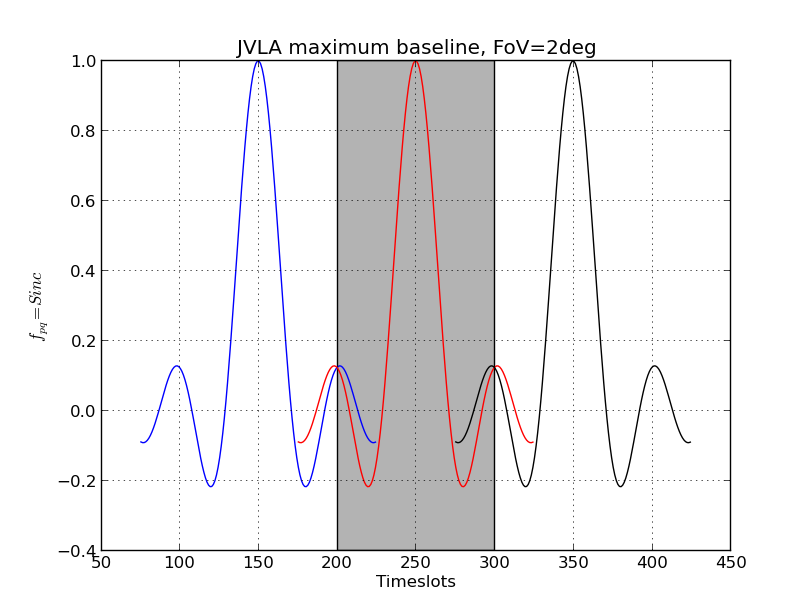
\includegraphics[width=1\textwidth]{./Figures/corrSigVLAMxBl_overlapLdelta.png}\caption{Overlap 
		\textit{BDWF's}: $\Delta_u t= [225, 250]$.}\label{ fig:fig_3a}\end{minipage}
\begin{minipage}{0.38\linewidth}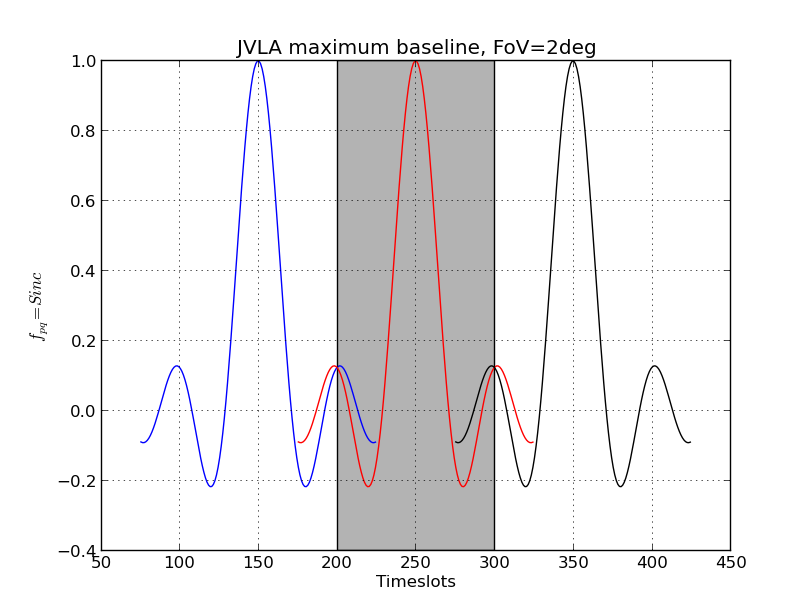
\includegraphics[width=1\textwidth]{./Figures/corrSigVLAMxBl_overlapLdelta.png}\caption{Overlap 
		\textit{BDWF's}: $\Delta_u t= [225, 250]$.}\label{ fig:fig_3a}\end{minipage}\\
\begin{minipage}{0.38\linewidth}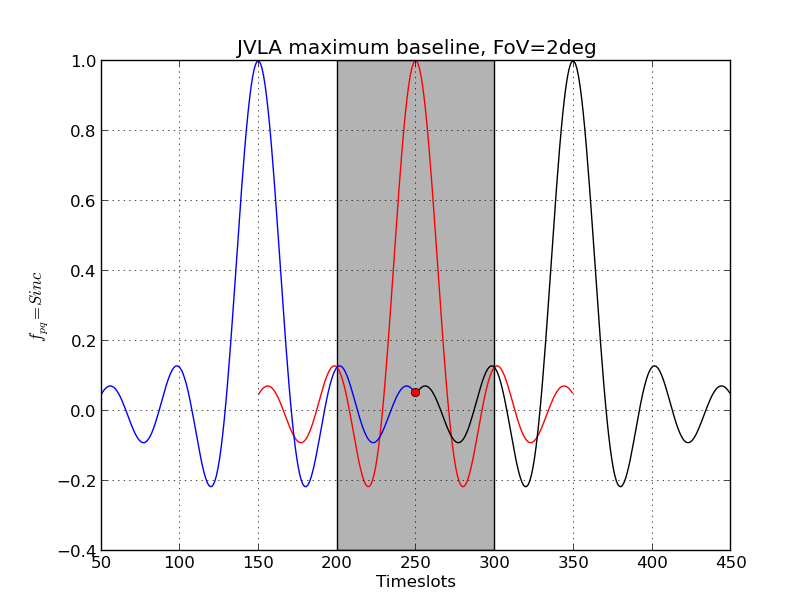
\includegraphics[width=1\textwidth]{./Figures/corrSigVLAMxBl.png}\caption{Overlap 
		\textit{BDWF's}: $\Delta_u t=\{250\}$.}\label{fig:fig_4}\end{minipage}
\begin{minipage}{0.38\linewidth}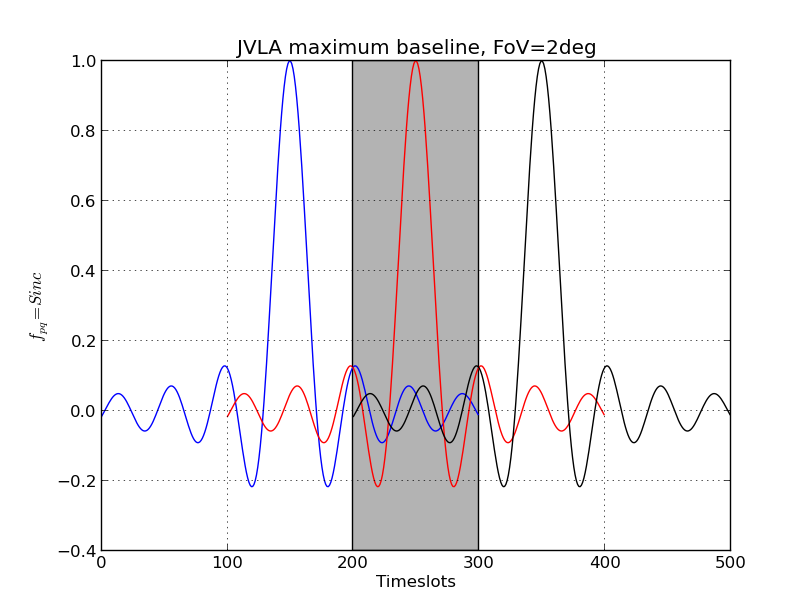
\includegraphics[width=1\textwidth]{./Figures/corrSigVLAMxBl_overlapGdelta.png}\caption{Overlap 
		\textit{BDWF's}: $\Delta_u t=\emptyset$.}\label{fig:fig_5}\end{minipage}
\end{figure*}
$1.)$ In Figures (\ref{fig1}) and (\ref{fig2}) we represented the ratio $\frac{\sigma_{meas,pq}}{\sigma_{av,pq}}$ as a function 
of $\sum_{i}^{n} u_i((t_c-t_i)/\lambda))$ ($\sigma_{meas,pq},\sigma_{av,pq}$ are the per baselines CWF and averaging rms noise  
respectively). We could also represented it as a function of baseline length. But, a uv-track corresponding to baseline aligned along the 
Est-West direction has longer tracts compare to one aligned along the South-Nordth for the same integration and frequency band. Therefore,  
$\frac{\sigma_{meas,pq}}{\sigma_{av,pq}}$ $v/s$ baselines length is ambiguous. We consider five baselines dependent 
windowing sinc function, $Bl$-$sinc$ $wk$ (with an extended width of $(k-1)n$ time intervals and/or frequency channels and $k \geq 1$). The 
experiment is done for two cases, figure (\ref{fig1}) is the one for $Bl$-$sinc$ $wk$ over both time-frequency and figure (\ref{fig2}) over 
time. These figures shows that, the noise increases with baselines length.\\

$2.)$ Figure (\ref{fig1}) shows that, with $Bl$-$sinc$ $wk$, the noise is lower on shorter baselines compared to the longer baselines. This 
is because on shorter  baselines  $\frac{\sigma_{meas,pq}}{\sigma_{av,pq}} \approx \frac{n}{n + k}$, it is the same case with 
Figure (\ref{fig2}) where $\frac{\sigma_{meas,pq}}{\sigma_{av,pq}} \approx \sqrt{\frac{n}{n + k}}$ (see the proof).  With $Bl$-$Sinc$ $wk$ 
($k>1$), the noise drops  with the extended number of time intervals and/or frequency channels of 
the window. The rate of this drop is non-linear with baselines length and also with the overlap time interval and/or frequency channels 
(see figure (\ref{fig1}b) and (\ref{fig2}b), the variation of the noise rate between baselines).  \\

$3.)$ In spite of the overlapping, with the theoretical results, the noise of longer baselines do not drop when the overlap 
samples is increased (figure \ref{fig2}). The reason is, few windows are overlapping in a visibility point when we extended in a unique 
direction (the time interval in this case) compare to two directions (time interval and frequency channels).
\begin{figure*}
 \centering
\begin{minipage}{0.38\linewidth}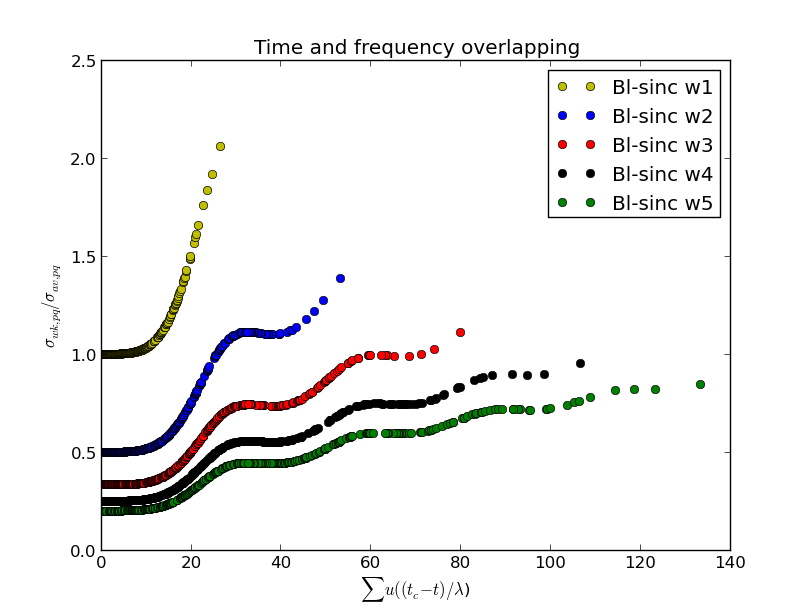
\includegraphics[width=1\textwidth]{./Figures/time_freq_ration.png}\caption{Noise ratio and rate 
of $Bl$-$sinc$-$wk$: time interval and frequency channels.}\label{ fig:fig_2a } \end{minipage}
\begin{minipage}{0.38\linewidth}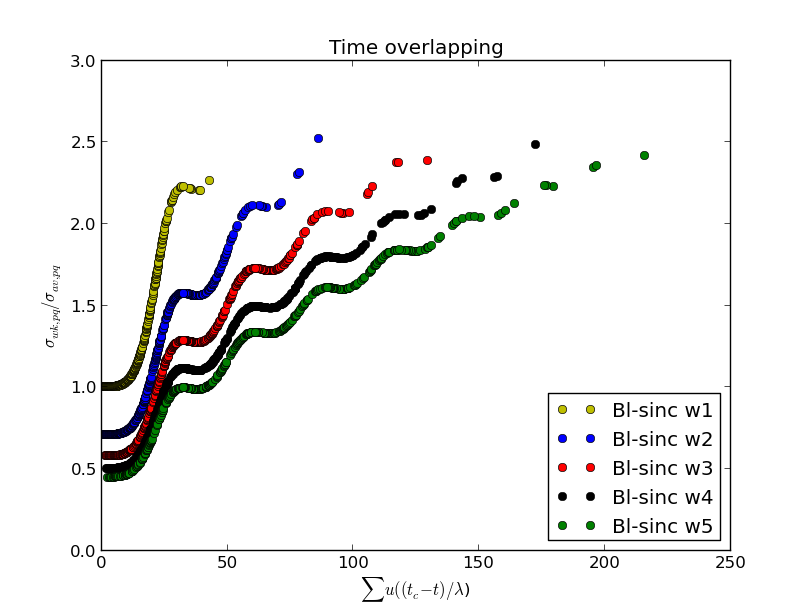
\includegraphics[width=1\textwidth]{./Figures/timeration.png}\caption{Noise ratio and rate of 
$Bl$-$sinc$-$wk$: time interval.}\label{fig:fig_2b}
\end{minipage}
\end{figure*} 
The theoretical derivation for the overall noise of $Bl$-$sinc$ $wk$ and the simulated one are quantified similarly but the pattern of the  
per baseline simulated rms noise do not look the same with the theoretical one. The number of $k$ determines the amount of noise  of CWF.
% \begin{table}
%  \begin{tabular}{|c|c|c|}
%   \textbf{Windows}&\textbf{\footnotesize theoretical analysis} &\textbf{\footnotesize simulation}\\
%   \hline\hline
%   { \footnotesize  }	  &{\footnotesize 1,066} & {\footnotesize 0,692}	\\ \cline{1-3}
% 	  
%   {\footnotesize } & {\footnotesize 1,334}& {\footnotesize 0,903} \\	\cline{1-3}
%   { \footnotesize  }	  &{\footnotesize 1,066} & {\footnotesize 0,692}	\\ \cline{1-3}
% 	  
%   {\footnotesize } & {\footnotesize 1,334}& {\footnotesize 0,903} \\	\cline{1-3}
%   { \footnotesize  }	  &{\footnotesize 1,066} & {\footnotesize 0,692}	\\ \cline{1-3}
% 	  
%   {\footnotesize } & {\footnotesize 1,334}& {\footnotesize 0,903} \\	\cline{1-3}
% \end{tabular}
% \caption{Theoretical and simulation results of the overall rms noise ratio : time interval and frequency channels.}
% \end{table}
% \pagebreak
% \begin{table}
%   \hspace{0cm}\begin{tabular}{|c|c|c|}
%   
%   \textbf{Windows}&\textbf{\footnotesize theoretical analysis} &\textbf{\footnotesize simulation}\\
%   \hline\hline
%   { \footnotesize  }	  &{\footnotesize 1,066} & {\footnotesize 0,692}	\\ \cline{1-3}
%     
%   {\footnotesize } & {\footnotesize 1,334}& {\footnotesize 0,903} \\	\cline{1-3}
%   { \footnotesize  }	  &{\footnotesize 1,066} & {\footnotesize 0,692}	\\ \cline{1-3}
% 	  
%   {\footnotesize } & {\footnotesize 1,334}& {\footnotesize 0,903} \\	\cline{1-3}
%   { \footnotesize  }	  &{\footnotesize 1,066} & {\footnotesize 0,692}	\\ \cline{1-3}
% 	  
%   {\footnotesize } & {\footnotesize 1,334}& {\footnotesize 0,903} \\	\cline{1-3}
% \end{tabular}
% \caption{Theoretical and simulation results of the overall rms noise ratio : time interval and frequency channels.}
% \end{table}
% \pagebreak
% \subsection{Analysis of $\mathcal{R}=\mathcal{F}^{-1}\{\mathcal{W}\}$}
% The CWF for each time interval  can be combined into a single two dimensional matrix,
% \begin{equation*}
% \mathcal{W}=
%   \begin{bmatrix}
%     W_{11} & W_{12} & \dots & W_{1n}\\
%     W_{21} & W_{22} & \dots & W_{2n}\\
%     \vdots & \vdots & \vdots & \vdots\\
%     W_{n1} & W_{n2} & \dots & W_{nn}\\
%   \end{bmatrix}
% \end{equation*}
\section{Simulation and results}
\section{Discussion}
\section{Conclusions}
\section*{Acknowledgments}
% 
% \subsection[]{Calibration}
% \label{sec:ALS}
% %Under the assumption of no noise: but we can already assume noise
% 
% In its general form, (unpolarized) calibration entails finding a diagonal antenna gain matrix $\GG=\rmn{diag}(\bmath{g})=$ 
% $\rmn{diag}([g_1,g_2,\cdots,g_n]^T)$ such that
% 
% \begin{equation}
% \label{eq:cal}
% ||\Rcal - \GG\Mcal\GG^H||
% \end{equation}
% 
% is minimized at each observational time-step.  The Hermitian matrix $\Rcal$ is the observed unpolarized visibility matrix, where element $r_{pq}$ of $\Rcal$ is the visibility measured by the baseline
% formed by antennas $p$ and $q$. The matrix $\Mcal$ is the corresponding visibility matrix generated from the calibration sky model. 
% Eq.~\ref{eq:cal} can then be restated as
% 
% \begin{equation}
% \label{eq:cal2}
% ||\Rcal-\bmath{g}\bmath{g}^H\odot\Mcal||=||\Rcal-\Gcal\odot\Mcal||,
% \end{equation}
% 
% where ``$\odot$'' represents element-by-element multiplication, and $\Gcal=\bmath{g}\bmath{g}^H$ is matrix product of the gain solution vector with its own Hermitian transpose. Crucially, $\Gcal$ is a rank one matrix by construction, and conversely, any rank one matrix can be decomposed into a product of the form $\bmath{g}\bmath{g}^H$.
% 
% Conventional approaches to radio interferometric calibration ignore the autocorrelations (i.e. the diagonal of the visibility matrix), since these are subject to a high additional self-noise term, and employ non-linear optimization techniques such as 
% Levenberg-Marquardt \citep{Levenberg1944,Marquardt1963} to find a maximum likelihood (ML) solution for the 
% off-diagonal terms of Eq.~\ref{eq:cal}. When a Gaussian noise model is assumed, this becomes 
% equivalent to least squares (LS) minimization: 
% 
% \begin{equation}
% \label{eq:LM}
% \min_{\bmath{g}} \sum_{p \neq q} (r_{pq} - g_p m_{pq} \conj{g}_q)^2, 
% \end{equation}
% 
% We will use the term LS calibration to refer to an LS solution of Eq.~\ref{eq:LM}. Most reduction packages in current use perform some sort of LS calibration. \citet{Kazemi2013a} propose an alternative approach called {\em robust calibration}, where a ML solution is obtained under the assumption of a $t$-distribution for the noise. Since implementations of robust calibration are not yet publicly available, we do not study it in this work. Where required, we make use of the MeqTrees package \citep{meqtrees} to do LS calibration.
% 
% %if the autocorrelation constraints are ignored. In \emph{MeqTrees}, Equation~\ref{eq:LM} is solved by using Levenberg-Marquardt \citep{Noordam2010}. %The term LS (Least Squares) calibration will be used to refer to the calibration approach that ignores the autocorrelation constraints (i.e. %Equation~\ref{eq:LM}). 
% 
% If autocorrelations are included in the optimization problem, an approach called Alternating Least Squares gain estimation \citep[ALS;][]{Boonstra2003,Wijnholds2009} can be used to obtain a solution to Eq.~\ref{eq:cal2}. It is not clear whether ALS provides a practical advantage over traditional LS without autocorrelations, since implementations of ALS compatible with conventional radio interferometric 
% data do not exist. The issue deserves to be investigated in a separate study. For our purposes, ALS turns out to provide a vital theoretical framework in which ghost formation can be understood analytically. 
% 
% \subsection{Ghost formation}
% \label{sec:ghostform}
% 
% In a nutshell, ghost sources are produced when Eq.~\ref{eq:cal} is solved for with an incomplete or incorrect model $\Mcal$. 
% Consider the simple case where the observed visibilities $\Rcal$ correspond to two point sources, and the 
% calibration model consists of a single point source at centre, $\Mcal=\bmath{1}$, where $\bmath{1}$ (boldface 1) represents a matrix of
% all ones (not a unity matrix!) 
% If we then assume a perfect instrument with unity gains, the actual solutions for $\GG$ will not be quite equal to unity, as they will attempt to fit for the difference between $\Mcal$ and $\Rcal$. Qualitatively, this process can be understood as follows: calibration attempts to move some ``real flux'' from the model $\Mcal$ to compensate for the unmodelled flux of the second point source. When these solutions are applied to the data, the resulting corrected visibilities
% 
% \begin{equation}
%   \Rcal^\mathrm{(c)} = \GG^{-1}\Rcal\GG^{-H},
%   \label{eq:corr}  
% \end{equation}
% 
% will contain ghost sources in addition to real sources. The rest of this paper analyses the mechanism by which this comes about. Note that we do not consider the effects of noise in our analysis; earlier empirical work \citep{Smirnov2010ghosts} has shown that the same pattern arises with or without noise.
% 
% In this context, LS calibration has proven to be very difficult to study theoretically. By contrast, the ALS formulation does yield the necessary insights. In this paper we therefore approach the problem of ghosts from several directions:
% 
% \begin{itemize}
%   \item We develop a theoretical framework based on ALS that predicts ghost formation;
%   \item We empirically compare the results of ALS and LS calibration, and show that they yield similar ghost patterns (with minor differences that are explained);
%   \item We provide empirical results for ghost formation using ALS and LS, and show that these match the theoretical predictions;
%   \item We show that all of the above match observed ghost patterns in real data, such as those seen in Fig.~\ref{fig:2004ghosts}.
% \end{itemize}
% 
% These results suggest that the theoretical insights gained from the ALS framework are valid for the LS approaches, while the last 
% point demonstrates that our simplified assumptions provide a good fit to real observations.
% 
% \subsection{Distillation}
% \label{sec:dist}
% 
% Since ghost sources are relatively faint (as we'll show below), they can be difficult to detect over the thermal noise and the PSF sidelobes of actual sources. In hindsight, this probably explains why the phenomena was not spotted earlier. A straightfoward way to detect the ghosts in simulations is to ``distill'' them into residual visibilities as follows:
% 
% \begin{enumerate}
%   \item We form predicted visibilities from a ``true'' sky ($\Mcal_0$), and an incomplete calibration sky model ($\Mcal$). 
%   \item The ``observed visibilities'' $\Rcal$ correspond to $\Mcal_0$ plus an optional noise term.
%   \item We obtain calibration solutions $\GG$ by solving Eq.~\ref{eq:cal} using $\Rcal$ and $\Mcal$.
%   \item We apply the solutions to $\Rcal$ (Eq.~\ref{eq:corr}), yielding corrected visibilities $\Rcal^\mathrm{(c)}$.   
%   \item We image the residuals $\Rcal^\Delta = \Rcal^\mathrm{(c)}-\Rcal$. The real sources then (mostly) cancel out, the noise term, if any, also (mostly) cancels out, and the resulting image yields the ``distilled'' ghost sources.
% \end{enumerate}
% 
% Note that in real-life observations, actual gains are never unity, and the residuals $\Rcal^\mathrm{(c)}-\Rcal$ would not reveal much since real sources would not cancel out. However, in our perfect telescope simulation, the gain solutions account for sky model incompleteness and nothing more, and the ghosts are easily visible in images of the residuals.
% 
% In the two-source, noise-free case considered here, the true sky $\Mcal_0$ is equal to
% 
% \[
%   \Rcal = \Mcal_0 = A_1 \bmath{1} + A_2 \bmath{K},
% \]
% 
% where $\bmath{K}$ is a Fourier kernel matrix of complex phase terms corresponding to the offset of the second source w.r.t. the phase centre. The residuals then correspond to 
% 
% \[
%   \Rcal^\Delta = A_1 \GG^{-1} \bmath{1} \GG^{-H} +  A_2 \GG^{-1} \bmath{K} \GG^{-H} - A_1 \bmath{1} - A_2 \bmath{K}
% \]
% 
% \newcommand{\Gtop}{\Gcal^{\top}}
% 
% By defining the matrix $\Gtop = \GG^{-1}\bmath{1}\GG^H$, we can rewrite this as
% 
% \[
%   \Rcal^\Delta = A_1 (\Gtop - \bmath{1}) + A_2(\Gtop - \bmath{1}) \odot \bmath{K}.
% \]
% 
% The matrix $\Gtop - \bmath{1}$ is in some sense fundamental. As will be shown below, it yields the basic ghost pattern corresponding to one source. From the equation above, we can see that the residuals will contain a superposition of two ghost patterns, scaled by $A_1$ and $A_2$, with the second pattern shifted to the position of the second source. In the general case, the residuals will correspond to a convolution of the true sky with $\Gtop - \bmath{1}$. Since in practice $A_2 \ll A_1$ (i.e. the missing flux in the model is usually considerably less than the flux accounted for), the first instance of the pattern is dominant (moreover, as will also be shown below, in the WSRT case the positions of the ghosts in the two patterns fall on top of one another). We shall refer to $\Gtop - \bmath{1}$ as the {\em distilled ghost pattern}.
% 
% 
% 
% \section[]{Theoretical derivation}
% 
% \label{sec:t_der}
% In this section analytic expressions for the elements of $\Gtop$ are derived. In the image domain each element of $\Gcal$ represents a different ghost pattern.
% The ghost patterns that are associated with $\Gcal$ form due to a loss of information. Since $\Gcal$ is of a lower rank than 
% $\Rcal$ (assuming a two source sky and a single source in the model) some information is lost when $\Gcal$ is computed. The inadequate rank one model $\Gcal$ leads to a significant change in the Fourier characteristics
% of the original matrix $\Rcal$. The change in Fourier characteristics manifest as ghost patterns when $\Gcal$ is imaged. 
% When $\Gtop$ is calculated the ghost patterns remain the same (the fluxes of the sources do however change). When the antenna gain solutions are applied
% to $\Rcal$ the ghost patterns of $\Gtop$ get convolved with the true sky, which implies that $\Rcal^\mathrm{(c)}$ will contain ghost sources. 
% The mathematical definition of a regularly-spaced array is given in Section~\ref{sec:conf}, while Section~\ref{sec:sky} gives a better description of the experimental test case that is considered. The analytic expressions for the elements of $\Gtop$ are then derived
% in Section~\ref{sec:ghost_p}.
% 
% \subsection[]{Regular and redundant array geometries}
% \label{sec:conf}
% 
% Since the geometric regularity of the WSRT layout will turn out to have an important effect on ghost formation, let's provide a formal mathematical definition here. 
% 
% \begin{definition}[Regularly-spaced array] Let us pick a coordinate system with origin at the first antenna position $\bmath{u}_0=0$.
% We shall call a set of antenna positions $\{\bmath{u}_p\}$ {\em regularly-spaced} if there exists a {\em common quotient baseline} (CQB) $\bmath{b}_0$ such that each antenna position is an integer multiple of $\bmath{b}_0$, i.e. that $\bmath{u}_p = \phi_p \bmath{b}_0$, with $\phi_p$ being a whole number. We will also require that $\bmath{b}_0$ is the largest such baseline (equivalently, the greatest common divisor of $\{\phi_p\}$ is 1).
% \end{definition}
% 
% \begin{definition}[Array geometry matrix]
% \label{def:phi}
% The array geometry matrix $\mathbf{\Phi}$ is an $n \times n$ integer matrix with elements $\phi_{pq}=\phi_q-\phi_p$. 
% \end{definition}
% 
% Ovbiously, a regularly-spaced array defined in this way is necessarily one-dimensional. Note that regularity is preserved under rotation. Note also that $\bmath{b}_0$ does not necessarily correspond to a real baseline. Most commonly-used configurations of the WSRT are regularly-spaced: the 10 fixed antennas have a CQB of 144m, while the CQB of the array as a whole is determined by the positions of the movable antennas RTA to RTD, with typical CQB lenghts of 6 or 12m\footnote{Since the WSRT movable antennas can in principle be placed at any position along a continuum, a non-regularly-spaced configuration is technically possible, but never used in practice.}. A {\em redundant} array will have many identical numbers in $\mathbf{\Phi}$. A regularly-spaced array is not necessarily redundant, but WSRT itself is highly redundant. 
% 
% The matrix $\mathbf{\Phi}$ has a few interesting mathematical properties, which will be fully derived in the Appendix. Note that the actual $uv$-coordinates of each baseline are given by $\bmath{b}_0\bmath{\Phi}$. The matrix $\bmath{\Phi}$ can be thought of as 
% representing a whole number scaling relationship between all the $uv$-tracks of the interferometer, and the {\em reference track} given by the CQB $\bmath{b}_0(t)$, which is a function of time due to the Earth's rotation. 
% 
% \subsection[]{The two source problem}
% \label{sec:sky}
% 
% Let us consider a sky composed of two unpolarized point sources of flux $A_1$ and $A_2$, and a calibration sky model consisting of just the primary source $A_1$. Since the solutions to the calibration equation (Eq.~\ref{eq:cal}) are invariant with respect to amplitude rescaling and positional shifts that are applied to both the sky and the model, we may, without loss of generality, restrict ourself to the case where the primary source has unity flux and is located at the phase centre. The ``true sky'' as a function of position $\bmath{s}=(l,m)$ (where $l$ and $m$ are the direction cosines) is then equal to 
% $I_{\mathcal{R}}(\bmath{s})=A_1\delta(\bmath{s})+A_2\delta(\bmath{s}-\bmath{s}_0),$ and the ``model sky'' to $I_{\mathcal{M}}(\bmath{s})=A_1\delta(\bmath{s})$, where $A_1 = 1$, $\bmath{s_0}=(l_0,m_0)\neq 0$ is the position of the secondary source, and $\delta$ is the Kronecker delta function. Let us further assume a perfect interferometer with unity gains, a monochromatic observation, and integration intervals sufficiently short to make smearing negligible. The 
% ``observed visibility'' corresponding to the true sky $I_{\Rcal}$ can be written as
% 
% \begin{equation}
% \label{eq:rtrue}
% r(\bmath{u}) = A_1 + A_2e^{-2\pi i \bmath{u}\cdot\bmath{s}_0},\\
% \end{equation}
% 
% where $\bmath{u}\cdot\bmath{s}_0$ is a dot product. If the array is regularly-spaced as defined above, then the visibility observed 
% by baseline $pq$ at $uv$-coordinates $\bmath{u}_{pq}=\phi_{pq}\bmath{b}_0$ is
% 
% \begin{equation}
% \label{eq:phi}
% V_{pq} = r(\bmath{u}_{pq}) = r(\phi_{pq}\bmath{b}_0) = A_1 + A_2e^{-2\pi i \phi_{pq}\bmath{b}_0\cdot\bmath{s}_0},\\
% \end{equation}
% where $\bmath{b}_0=\bmath{b}_0(t)$ is the CQB. The ``model visibilities'' corresponding to the model sky $I_{\Mcal}$ above, are trivially all unity.
% 
% \subsection[]{The extrapolated visibilities matrix}
% \label{sec:ghost_p}
% The observed visibilities for each observational time step can be packed into a two dimensional matrix 
% \begin{equation}
% \Rcal = \left[ \begin{array}{cccc}
% V_{11} & V_{12} & \cdots & V_{1n}\\
% V_{21} & V_{22} & \cdots & V_{2n}\\
% \vdots&\vdots&\vdots&\vdots\\
% V_{n1} & V_{n2} & \cdots & V_{nn}\end{array} \right].
% \end{equation} 
% The elements of $\Rcal$ are functions that depend on time. For a regularly-spaced array, Equation~\ref{eq:phi} can be utilized to rewrite all the elements of $\Rcal$ as functions of $\bmath{b}_0$. We can express this formally via the following definition:
% 
% \begin{definition}[Extrapolated visibilities matrix]
% \label{def:R}
% Let $\Rcal(\bmath{b})$ be an $n \times n$ Hermitian function-valued matrix with entries
% \begin{equation}
% \label{eq:rpq}
% r_{pq}(\bmath{b}) = r(\phi_{pq}\bmath{b}),
% \end{equation}
% where $r$ is given by Equation~\ref{eq:rtrue}, $\phi_{pq}$ is given by the array geometry matrix $\mathbf{\Phi}$, $\bmath{b}=(u,v)$ and 
% $\bmath{s}_0=(l_0,m_0)\neq 0$ are real two-vectors, $A_1=1$, and $0<A_2<1$.\\ 
% \end{definition}
% 
% This allows us to formally define $\Rcal(\bmath{b})$ over the entire $uv$-plane, i.e. for any value $\bmath{b}$. The actual observed visibilities $\Rcal$ at time $t$ are given by $\Rcal(\bmath{b}_0(t))$. For any given baseline $pq$, $r_{pq}(\mathbf{b}_0)$ corresponds to the visibilities measured by that baseline. Since $\bmath{b}_0(t)$ follows an elliptical track, our actual ``measurements'' on baseline $pq$ (i.e. the values subject to calibration) are restricted to that series of $uv$-points. However, by replacing $\bmath{b}_0$ by the free variable $\bmath{b}$ in Equation~\ref{eq:rpq}, we automatically define an ``extrapolated'' visibility function over the entire $uv$-plane. By definition, the values of $r_{pq}$ over the track $\bmath{b}_0(t)$ are equal to visibilities measured by baseline $pq$ over the track $\phi_{pq}\bmath{b}_0(t)$. 
% 
% Extrapolation, as defined above, forms the crux of the following derivations. 
% 
% Note also that Equation~\ref{eq:rpq} can also be seen as a coordinate scaling relationship between the observed visibility distribution $r(\bmath{u})$ and any given $r_{pq}(\bmath{b})$. To emphasize this, we use the variable $\bmath{u}$ to represent coordinates in the  ``observed'' $uv$-plane (where $r$ lives), and $\bmath{b}$ for coordinates in the ``scaled'' $uv$-planes (where the $r_{pq}$'s live). This also implies that the ``sky'' corresponding to any $r_{pq}$ (i.e. the inverse Fourier tranasform of $r_{pq}$) is a ``scaled up'' version of the true sky:
% 
% \begin{equation}
% \label{eq:skyscaling}
% I_{pq}(\bmath{s}) = \Fcal^{-1}\{r_{pq}\}(\bmath{s}) = I_{\Rcal} \bigg(\frac{\bmath{s}}{\phi_{pq}} \bigg).
% \end{equation}
% 
% Finally and most crucially, the $\Rcal(\bmath{b})$ matrix for any $\bmath{b}\neq 0$ can be shown to have rank two (see Proposition~\ref{prop:1} in the Appendix). 
% 
% \subsection[]{The calibration matrix}
% 
% Since our model visibilities are all unity, the calibration process (Equation~\ref{eq:cal2}) entails finding some kind of ``best fit'' 
% rank one matrix $\Gcal$, given $\Rcal$. In effect, the calibration process results in a mapping $\Rcal\to\Gcal$; by extension, this also defines a mapping $\Rcal(\bmath{b})\to\Gcal(\bmath{b})$ for any $\bmath{b}$. For LS calibration, the best fit is given by Equation~\ref{eq:LM}. This has proven difficult to explore analytically, so we will consider ALS calibration instead (and later empirically show that it yields similar results).
% 
% In a nutshell, ALS calibration obtains a $\Gcal$ by ``de-ranking'' $\Rcal$, i.e. keeping just its largest eigenvalue. More precisely:
% 
% \begin{definition}[ALS calibration matrix]
% \label{def:G}
% Let $\Gcal(\bmath{b})=\lambda(\bmath{b})\mathbf{x}(\bmath{b})\mathbf{x}^{H}(\bmath{b})$, where $\lambda(\bmath{b})$ is the largest eigenvalue of $\Rcal(\bmath{b})$, and $\mathbf{x}(\bmath{b})$
% is its associated normalized eigenvector.\\
% \end{definition}
% 
% We will designate the elements of $\Gcal$ as $g_{pq}(\bmath{b})$.
% 
% To provide a specific example of the above, let us create a theoretical three-element interferometer with a geometry matrix of
% \begin{equation}
% \mathbf{\Phi}=\left[ \begin{array}{ccc}
% 0 & 3 & 5\\
% -3 & 0 & 2\\
% -5& -2 & 0 \end{array} \right],
% \end{equation}
% 
% \begin{figure}
%  \centering
%  \includegraphics[width=0.48\textwidth]{./V_R_G_12.pdf}
%  % V_R_3.pdf: 585x441 pixel, 72dpi, 20.64x15.56 cm, bb=0 0 585 441
%  \caption{The functions $r_{12}(\bmath{b})$ and $g_{12}(\bmath{b})$.}
%  \label{fig:fig1} 
% \end{figure}
% \begin{figure}
%  \centering
%  \includegraphics[width=0.48\textwidth]{./V_R_G_13.pdf}
%  % V_R_3.pdf: 585x441 pixel, 72dpi, 20.64x15.56 cm, bb=0 0 585 441
%  \caption{The functions $r_{13}(\bmath{b})$ and $g_{13}(\bmath{b})$.}
%  \label{fig:fig2} 
% \end{figure}
% \begin{figure}
%  \centering
%  \includegraphics[width=0.48\textwidth]{./V_R_G_23.pdf}
%  % V_R_3.pdf: 585x441 pixel, 72dpi, 20.64x15.56 cm, bb=0 0 585 441
%  \caption{The functions $r_{23}(\bmath{b})$ and $g_{23}(\bmath{b})$.}
%  \label{fig:fig3} 
% \end{figure}
% 
% and place a secondary source of flux $A_2=0.2$Jy at $l_0=1^{\circ},m_0=1^{\circ}$. Fig.~\ref{fig:fig1}, Fig. ~\ref{fig:fig2} and Fig. ~\ref{fig:fig3} graphically display the resulting $\Rcal(\bmath{b})$ and $\Gcal(\bmath{b})$ matrices. The following observations can also be made. The functions $r_{pq}(\bmath{b})$ are trivial phase gradients, and are thus continuous, Hermitian and periodic in 
% the $u$ and $v$ direction with periods of  $\frac{1}{\phi_{pq}|l_0|}$ and $\frac{1}{\phi_{pq}|m_0|}$. They are effectively one-dimensional,
% i.e. constant along each line $v=-\frac{l_0}{m_0}u+c$ for any $c$. The $\Gcal(\bmath{b})$ functions have a more interesting structure, but are also continuous, Hermitian, one-dimensional and periodic, with periods along $u$ and $v$ of $\frac{1}{|l_0|}$ and $\frac{1}{|m_0|}$. Moreover, this holds for any ALS calbiration matrix as defined above (see Proposition~\ref{prop:2}). The difference between the $g_{pq}$'s is that 
% each of them has a different secondary harmonic which is determined by $\phi_{12},\phi_{13}$ and $\phi_{23}$.
% 
% Any periodic, one-dimensional function can be written out in terms of a one-dimensional discrete Fourier transform. We can therefore decompose each $g_{pq}$ as follows:
% 
% \begin{equation}
% \label{eq:m_v}
% g_{pq}(\bmath{b}) = \sum_{j=-\infty}^{\infty}c_{j,pq}^{\mathcal{G}}e^{2\pi i j\bmath{b}\cdot\bmath{s}_0}
% \end{equation}
% 
% Proposition~\ref{prop:3} derives this result formally. The coefficients $c_{j,pq}^{\mathcal{G}}$ (real, since $g_{pq}$ is Hermitian) 
% have a very non-trivial structure, but they can be calculated using Equation~\ref{eq:eq_2}. 
% 
% Now, since $g_{pq}(\bmath{b})$ represents the predicted corrupted visibilities (given that we have a unity model), it is fair to ask, what 
% image-plane distribution corresponds to the visiblitity distribution $g_{pq}(\bmath{b})$? Doing an inverse 2D Fourier transform, we obtain:
% 
% \begin{equation}
% \Fcal^{-1}\{\ g_{pq} \}(\bmath{s}) = \sum_{j=-\infty}^{\infty}c_{j,pq}^{\mathcal{G}}\delta(\bmath{s}+j\bmath{s}_0),
% \end{equation}
% 
% i.e. a sum of delta-functions whose locations are integer multiples of $\bmath{s}_0=(l_0,m_0)$. 
% 
% Let us now define something we'll call the ``$\Gcal$-sky of baseline $pq$'' as follows:
% 
% \begin{eqnarray*}
% I_{pq}^{\mathcal{G}}(\bmath{s}) &=& \mathcal{F}^{-1}\bigg\{\ g_{pq}\bigg(\frac{\bmath{b}}{\phi_{pq}}\bigg) \bigg\}\\
% \label{eq:IpqG}
% &=&\sum_{j=-\infty}^{\infty}c_{j,pq}^{\mathcal{G}}\,\delta\bigg(\bmath{s}+\frac{j \bmath{s}_0}{\phi_{pq}}\bigg). 
% \end{eqnarray*}
% 
% The physical meaning of $I_{pq}^{\mathcal{G}}$ is as follows: it is a sky distribution whose Fourier transform yields a visibility
% distribution that, along the track $\phi_{pq}\bmath{b}_0(t)$, is consistent with the \emph{predicted corrupted visibilities} $g_{pq}$ along the track given by $\bmath{b}_0(t)$ (note how the scaling relationship of Equation~\ref{eq:rpq} enters into Equation~\ref{eq:IpqG}).  In other words, after the best-fitting calibration gains have been applied, the resulting predicted visibilities for each baseline $pq$ {\em will be consistent with a sky of delta functions spaced at intervals of} $s_0/\phi_{pq}$, with intensities given by $\{c_{j,pq}^{\mathcal{G}}\}$.
% 
% These delta functions are the fundamental ingredients of the ghosts observed in Fig.~\ref{fig:2004ghosts}. We will shortly show that the corrected visibilities exhibit a similar structure, but first let us consider what happens to the visibilies given by $g_{pq}$ during imaging.
% 
% \subsection{Imaging}
% 
% In the situation above, each baseline's predicted corrupted visibilities correspond to its own apparent sky $I_{pq}$. During conventional interferometric imaging, the per-baseline visibilities are interpolated onto a ``common'' $uv$-plane using convolutional gridding, and the result is Fourier transformed back into an estimate of the sky (the so-called ``dirty image''). Mathematically, this can be described as follows: 
% 
% \begin{equation}
% I_D = \mathcal{F}^{-1}\bigg\{\ \sum_{pq} S_{pq}\mathcal{F}\{ I_{pq} \}\ \bigg\}. 
% \end{equation}
% 
% Here, $S_{pq}$ is the \emph{sampling function} of baseline $pq$. The sampling function is only non-zero in the neighbourhood of the track described by $\bmath{u}_{pq}$, and accounts for both the imaging weights and the interpolation coefficients of the gridding process. This can be rewritten as
% 
% \begin{equation}
% \label{eq:Idpq}
% I_D = \sum_{pq} P_{pq} \circ I_{pq}, 
% \end{equation}
% where $P_{pq}=\mathcal{F}\{S_{pq}\}$ is the (unnormalized) PSF associated with baseline $pq$. Note that in the case of each baseline seeing a common sky $I$, the above becomes
% \begin{equation}
% I_D = (\sum_{pq} P_{pq} ) \circ I, 
% \end{equation}
% which is the familiar result that the dirty image $I_D$ is the convolution of the true sky $I$ by the point spread function of the array $P$ given by
% \begin{equation}
% \label{eq:psf}
% P = \sum_{pq} P_{pq}.
% \end{equation}
% 
% Now, recall that Equation~\ref{eq:IpqG} describes a string of delta functions spaced at intervals of $\bmath{s}_0/\phi_{pq}$. 
% If we define $\phi_0$ as the least common multiple of all $\phi_{pq}$, we can rewrite the equation as a sequence of delta functions spaced
% at intervals of $\bmath{s}_0/\phi_0$, some of them possibly of zero amplitude: 
% 
% \begin{eqnarray*}
% \label{eq:IpqG1}
% I_{pq}^{\mathcal{G}}(\bmath{s}) 
% = \sum_{k=-\infty}^{\infty}d_{k,pq}^{\mathcal{G}}\,\delta\bigg(\bmath{s}+\frac{k \bmath{s}_0}{\phi_0}\bigg),
% \end{eqnarray*}
% 
% where $d_{k,pq}^{\mathcal{G}}=c_{j,pq}^{\mathcal{G}}$ if $k$ is evenly divisible by $\phi_{pq}$ (with $j=k/\phi_{pq}$), and zero otherwise. To simplify further equations, we'll use the $\delta_k$ as shorthand for the $k$-th delta function above:
% 
% \[
% \delta_k(\bmath{s}) = \delta\bigg(\bmath{s}+\frac{k \bmath{s}_0}{\phi_0}\bigg).
% \]
% 
% Substituting this into Equation~\ref{eq:Idpq}, we get
% \begin{eqnarray*}
% I_D^\mathcal{G} &=& \sum_{pq} P_{pq} \circ \bigg ( \sum_{k=-\infty}^{\infty}d_{k,pq}^{\mathcal{G}}\,\delta_k\bigg) \\
% \label{eq:ID}
%  &=& \sum_{k=-\infty}^{\infty} \bigg ( \sum_{pq} d_{k,pq}^{\mathcal{G}}P_{pq} \bigg ) \circ \delta_k.
% \end{eqnarray*}
% 
% Physically, this can be interpreted as follows. The dirty image $I_D^\mathcal{G}$ which we get as a result of imaging the predicted corrupted visibilities consists of a string of delta functions at regularly-spaced locations $k \bmath{s}_0/\phi_0$, each one convolved with its own {\em ghost spread function} (GSF) $P^\mathcal{G}_k$:
% 
% \begin{equation}
% \label{eq:gsf}
% P^\mathcal{G}_k = \sum_{pq} d_{k,pq}^{\mathcal{G}}P_{pq}.
% \end{equation}
% 
% Comparing this to Equation~\ref{eq:psf}, we can now understand the previously puzzling observation that the ghost sources in Fig.~\ref{fig:2004ghosts} appear to be convolved with differing point spread functions, similar but not identical to the nominal PSF of
% the WSRT.
% 
% \subsection{Corrected visibilities}
% 
% In real life, one would typically be imaging the \emph{corrected visibilities} (Sect.~\ref{sec:ghostform}) given by
% 
% \begin{equation}
% \label{eq:cor}
%  \Rcal^\mathrm{(c)} = \GG^{-1}\Rcal\GG^{-H} = \Gcal^{\top}\odot\Rcal,
% \end{equation}
% 
% and our real goal is to understand the effect of $\Gcal$ on the \emph{corrected sky} $I^\mathrm{(c)} = \Fcal^{-1}\{\Rcal^\mathrm{(c)}\}$. To get there, we need to take an intermediate step. First, let us define  a ``$\Gcal^\top$-sky'' whose Fourier transform is consistent with the visibility distribution given by $g_{pq}^{-1}$. Proposition~\ref{prop:4} shows\footnote{Note that this proposition implicitly assumes
% $g_{pq}\neq 0$, i.e. that the ALS calibration solutions are not null. Intuition suggests that this is a safe assumption: a null gain solution would yield null predicted visibilities, which could hardly be a ``best fit'' to the calibration equation in any sense. However, obtaining a rigorous proof of this has been surprisingly difficult, so we will let the assumption stand as is.} that the visibility distribution $g^{-1}_{pq}(\bmath{b})$ can also be decomposed into a Fourier series:
% 
% \begin{equation}
% \label{eq:m_v}
% g^{-1}_{pq}(\bmath{b}) = \sum_{j=-\infty}^{\infty}c^\top_{j,pq} e^{2\pi i j\bmath{b}\cdot\bmath{s}_0},
% \end{equation}
% 
% which implies that the corresponding ``$\Gcal^\top$-sky'' has a similar form to Equation~\ref{eq:IpqG1}, but with a different set of coefficients:
% 
% \begin{equation}
% \label{eq:G_inv}
% I_{pq}^{\mathcal{G}^{\top}} = \sum_{k=-\infty}^{\infty}d_{k,pq}^{\top}\,\delta_k.
% \end{equation}
% 
% Now, consider the matrix $\Gcal^\top(\bmath{b}) \odot \Rcal(\bmath{b})$. We'll designate its elements as $r_{pq}^\top(\bmath{b})$. The inverse Fourier transform of each element is then 
% 
% \begin{equation}
% \mathcal{F}^{-1}\{ r_{pq}^\top \} = \mathcal{F}^{-1}\{ g^{-1}_{pq} \} \circ \mathcal{F}^{-1}\{ r_{pq} \},
% \end{equation}
% 
% and the inverse Fourier transforms of both components have already been derived above. This means that the ``corrected sky'' 
% corresponding to the corrected visibilities of baseline $pq$ is given by
% 
% \begin{equation}
% I_{pq}^\mathrm{(c)} = I_{pq}^{\mathcal{G}^{\top}} \circ I^{\mathcal{R}},
% \end{equation}
% % 
% i.e. is simply a convolution of the real sky $I^{\mathcal{R}}$ with the ``ghost pattern'' of delta functions given by $I_{pq}^{\mathcal{G}^{\top}}$ above. In other words, the ``corrected sky'' will contain multiple instances of the fundamental ghost 
% pattern (what we call the distilled ghost pattern), centered on each source, and scaled by the flux of that source. It is also easy to see that the sky corresponding to the residuals $\Rcal^\Delta$ is given by
% 
% \begin{equation}
% \label{eq:IpqDelta}
% I_{pq}^\Delta = I_{pq}^{\mathcal{G}^{\top}\!-1} \circ I^{\mathcal{R}} = (I_{pq}^{\mathcal{G}^{\top}}-\delta) \circ I^{\mathcal{R}}.
% \end{equation}
% 
% The $I_{pq}^{\mathcal{G}^{\top}\!-1}$ term is the per-baseline sky associated with the distilled ghost pattern $\Gcal^\top-\bmath{1}$. 
% By analogy with Equation~\ref{eq:ID}, we can derive an expression for the full dirty image:
% 
% \begin{equation}
% \label{eq:IdGT1}
% I_D^{\mathcal{G}^{\top}\!-1} = \sum_{k=-\infty}^{\infty} \bigg ( 
% \sum_{pq} \hat{d}_{k,pq}^{\top} P_{pq} 
% \bigg ) \circ \delta_k,
% \end{equation}
% 
% where $\hat{d}_{k,pq}^\top = d_{k,pq}^\top-1_{\{k=0\}}$, and the notation $1_{\{k=0\}}$ represents a series whose coefficients 
% are 1 at $k=0$ and 0 elsewhere. Note the physical meaning of this operation: the $d_{0,pq}^\top$ coefficient corresponds to the
% position of the real source $A_1$ in the image, and is close to unity, since the corrected visibilities contain the real source 
% as well as all the ghosts. Subtracting 1 from this corresponds to taking the residual visibilities.
% 
% In our simple case the real sky consists of two sources, and the resulting corrected sky is a superposition of 
% two patterns given by $I_{pq}^{\mathcal{G}^{\top}}$, scaled by $A_1$ and $A_2$, and centered on origin and on $\bmath{s}_0$, 
% respectively. Since each pattern yields ghosts at discrete intervals of $\bmath{s}_0/\phi_{0}$, the two sets of positions
% align, and we can work out the amplitudes of the resulting superposed ghost sources by summing up the corresponding coefficients. 
% By analogy with Equation~\ref{eq:ID}, we can derive the following equation for the dirty image formed from corrected visibilities:
% 
% \begin{equation}
% \label{eq:Idcorr}
% I_D^\mathrm{(c)} = \sum_{k=-\infty}^{\infty} \bigg ( 
% \sum_{pq} (A_1d_{k,pq}^\top + A_2d_{k-\phi_0,pq}^\top)
% P_{pq} 
% \bigg ) \circ \delta_k.
% \end{equation}
% 
% From Equation~\ref{eq:IpqDelta}, it follows that the dirty image corresponding to the residuals can be obtained by subtracting unity from the corresponding $d$ coefficient:
% 
% \begin{equation}
% \label{eq:Idres}
% I_D^\Delta = \sum_{k=-\infty}^{\infty} \bigg ( 
% \sum_{pq} (A_1 \hat{d}_{k,pq}^\top + A_2 \hat{d}_{k-\phi_0,pq}^\top)
% P_{pq} 
% \bigg ) \circ \delta_k,
% \end{equation}
% 
% where again $\hat{d}_{k,pq}^\top=d_{k,pq}^\top-1_{\{k=0\}}$.
% 
% Equations~\ref{eq:ID}, \ref{eq:IdGT1}, \ref{eq:Idcorr} and \ref{eq:Idres} summarize the formation of ghost patterns in the predicted corrupted, corrected and residual visibilities. 
% 
% For our purposes, it is important to derive a theoretical prediction for the amplitudes of individual ghost sources as a 
% fraction of the ``missing flux'' $A_2$. Consider the $k$-th ghost source located at $k\bmath{s}_0/\phi_0$. 
% From Equation~\ref{eq:IdGT1}, it follows that the amplitude of the ghost source is given by the weighted sum
% 
% \[
% \sum_{pq} \hat{d}_{k,pq}^{\top} P_{pq}(0), 
% \]
% 
% where the per-baseline weights $P_{pq}(0)$ are ultimately determined by the imaging weights. For simplicity, let us consider the case of natural weighting, in which case the sum becomes unweighted. We can then define the quantity
% 
% \newcommand{\pqavg}[1]{\left\langle#1\right\rangle_{pq}}
% 
% \begin{equation}
% \zeta_k^{\mathcal{G}^{\top}\!-1} =\frac{\pqavg{\hat{d}_{k,pq}^{\top}}}{A_2}, 
% \end{equation}
% 
% where $\pqavg{\cdot}$ denotes averaging over all baselines $pq$. This gives us the amplitude of the $k$-th ghost source in the distilled pattern, as a fraction of $A_2$ (assuming natural weighting), and can be computed analytically from the results above. Likewise,
% the $k$-th source in the corrected residuals is a superposition of two sources from the distilled pattern, and its amplitude as a fraction of $A_2$ is given by (assuming natural weighting):
% 
% \begin{eqnarray*}
% \zeta_k^\Delta &=& \frac{\pqavg{A_1 \hat{d}_{k,pq}^\top + A_2 \hat{d}_{k-\phi_0,pq}^\top}}{A_2} \\
% \label{eq:zeta}
% &=& \frac{A_1}{A_2} \pqavg{\hat{d}_{k,pq}^\top} + \pqavg{\hat{d}_{k-\phi_0,pq}^\top}
% \end{eqnarray*}
% 
% 
% Of particular interest is the quantity $\zeta_{\phi_0}^\Delta$, as this gives the relative amplitude of the ``flux suppression ghost''
% sitting on top of source $A_2$. Indirectly, this one ghost 
% has been observed since the invention of selfcal, since it corresponds to the well-known phenomenon of flux suppression in unmodelled sources. The theoretical derivation given here provides an explanation for this.
% 
% % where $\gamma_{j,pq}^{\mathcal{G}^{\top}\!\!\odot\mathcal{R}} = A_1 \alpha_{j,pq} + A_2 \beta_{j,pq}$, $\alpha_{j,pq} = c_{j,pq}^{\mathcal{G}^{\top}}$, $\beta_{j,pq}=c_{j+\phi_{pq},pq}^{\mathcal{G}^{\top}}$ and
% % ``$\star$'' represents covolution. Note that the coefficients in Equation~\ref{eq:f_eq} can be indexed with $j$ or $\bmath{s}$, where $\bmath{s}=\left\langle -\frac{jl_0}{\phi_{pq}}, -\frac{jm_0}{\phi_{pq}}\right\rangle$. 
% 
% % Similarly,
% % \begin{eqnarray*}
% % \label{eq:one}
% % \gamma_{j,pq}^{\mathcal{G}^{\top}\!\!\odot\hat{\mathcal{R}}} &=& A_p \alpha_{j,pq} + A_s \beta_{j,pq},\\
% % \gamma_{j,pq}^{\mathcal{G}^{\top}\!-1} &=& \hat{\alpha}_{j,pq},\\
% % \gamma_{j,pq}^{(\mathcal{G}^{\top}\!-1)\odot\hat{\mathcal{M}}} &=& A_p\hat{\alpha}_{j,pq},\\
% % \gamma_{j,pq}^{(\mathcal{G}^{\top}\!-1)\odot\mathcal{R}} &=& A_1 \hat{\alpha}_{j,pq} + A_2 \hat{\beta}_{j,pq},\\
% % \label{eq:four}
% % \gamma_{j,pq}^{(\mathcal{G}^{\top}\!-1)\odot\hat{\mathcal{R}}} &=& A_p \hat{\alpha}_{j,pq} + A_s \hat{\beta}_{j,pq}\\
% % \mathbfss{E}_{pq}[\gamma_{\bmath{s},pq}^{\mathcal{G}^{\top}\!-1}] &=& \mathbfss{E}_{pq}[\hat{\alpha}_{\bmath{s},pq}],\\
% % \mathbfss{E}_{pq}[\gamma_{\bmath{s},pq}^{(\mathcal{G}^{\top}\!-1)\odot\hat{\mathcal{M}}}] &=& A_p\mathbfss{E}_{pq}[\hat{\alpha}_{\bmath{s},pq}],\\
% % \mathbfss{E}_{pq}[\gamma_{\bmath{s},pq}^{(\mathcal{G}^{\top}\!-1)\odot\mathcal{R}}] &=& A_1 \mathbfss{E}_{pq}[\hat{\alpha}_{\bmath{s},pq}] + A_2 \mathbfss{E}_{pq}[\hat{\beta}_{\bmath{s},pq}],\\
% % \mathbfss{E}_{pq}[\gamma_{\bmath{s},pq}^{(\mathcal{G}^{\top}\!-1)\odot\hat{\mathcal{R}}}] &=& A_p \mathbfss{E}_{pq}[\hat{\alpha}_{\bmath{s},pq}] + A_s \mathbfss{E}_{pq}[\hat{\beta}_{\bmath{s},pq}],
% % \end{eqnarray*}
% % where $\hat{\alpha}_{j,pq} = \alpha_{j,pq} - 1_{\{j=0\}}$, $\hat{\beta}_{j,pq} = \beta_{j,pq} - 1_{\{j=-\phi_{pq}\}},\hat{\alpha}_{\bmath{s},pq} = \alpha_{\bmath{s},pq} - 1_{\{\bmath{s}=\bmath{0}\}}$, $\hat{\beta}_{\bmath{s},pq} = \beta_{\bmath{s},pq} - 1_{\{\bmath{s}=\bmath{s}_0\}}$ and $\mathbfss{E}_{pq}[]$ represents the sample average taken over
% % all baselines.    
% % Useful quantities to consider are 
% % \begin{equation}
% % \label{eq:m1}
% % \zeta_{\bmath{s},pq}^{\mathcal{G}^{\top}\!-1}=\bigg|\frac{\mathbfss{E}_{pq}[\gamma_{\bmath{s},pq}^{\mathcal{G}^{\top}\!-1}]}{A_2}\bigg|,
% % \end{equation}
% % and
% % \begin{equation}
% % \label{eq:m2}
% % \zeta_{\bmath{s},pq}^{(\mathcal{G}^{\top}\!-1)\odot\mathcal{R}}=\bigg|\frac{\mathbfss{E}_{pq}[\gamma_{\bmath{s},pq}^{(\mathcal{G}^{\top}\!-1)\odot\mathcal{R}}]}{A_2}\bigg|. 
% % \end{equation}
% % Equation~\ref{eq:one}--\ref{eq:m2} will play a prominent role in Section~\ref{sec:results}. Notice that
% % \begin{equation}
% % \bigg|\frac{\mathbfss{E}_{pq}[\gamma_{\bmath{s},pq}^{\mathcal{G}^{\top}\!-1}]}{A_2}\bigg| \equiv \bigg|\frac{\mathbfss{E}_{pq}[\gamma_{\bmath{s},pq}^{(\mathcal{G}^{\top}\!-1)\odot\hat{\mathcal{M}}}]}{A_s}\bigg|,
% % \end{equation} 
% % and
% % \begin{equation}
% % \bigg|\frac{\mathbfss{E}_{pq}[\gamma_{\bmath{s},pq}^{(\mathcal{G}^{\top}\!-1)\odot\mathcal{R}}]}{A_2}\bigg| \equiv \bigg|\frac{\mathbfss{E}_{pq}[\gamma_{\bmath{s},pq}^{(\mathcal{G}^{\top}\!-1)\odot\hat{\mathcal{R}}}]}{A_s}\bigg|,
% % \end{equation}
% % which reafirms the validity of the no loss of generality assumption that was made in Section~\ref{sec:sky}.
% 
% % % Equation~\ref{eq:f_eq} implies that applying the gain solutions to
% % % $\Rcal$ generates spurious point sources for each baseline. Moreover, the distribution pattern of these spurious point sources differ for each baseline and is mainly determined
% % % by the dependence factor $\phi_{pq}$. The ghost point sources of each baseline $pq$ lie on the discrete line $m = \frac{m_0}{l_0}l$, where $l=\frac{jl_0}{\phi_{pq}};j\in\mathbfss{Z}$.
% 
% % % When either $l_0 = 0^{\circ}$ or $m_0 = 0^{\circ}$ the above derivation simplifies and becomes one dimensional.
% 
% % %\subsection[]{Source suppression}
% % %Some of the flux of the secondary source gets modeled by $\Gcal(\bmath{b})$. It is therefore only logical that applying the gain solution to $\Rcal(\bmath{b})$ will
% % %suppress the flux of the secondary source. The flux in the secondary source that remain after applying the gain solution can be derived with Equation~\ref{eq:cor} and is equal
% % %to 
% % %\begin{equation}
% % %A_2^{r_{pq}} =  |l_0||m_0|\int_{-\frac{1}{2|m_0|}}^{\frac{1}{2|m_0|}}\int_{-\frac{1}{2|l_0|}}^{\frac{1}{2|l_0|}}\frac{V_{pq}^{\mathcal{R}}(u,v)}{V_{pq}^{\mathcal{G}}(u,v)}e^{2\pi i \phi_{pq} \bmath{b}\cdot\bmath{s}_0}~dudv
% % %\end{equation}
% % %Similarly the flux in the primary source that remain after calibration is equal to
% % %\begin{equation}
% % %A_1^{r_{pq}} =  |l_0||m_0|\int_{-\frac{1}{2|m_0|}}^{\frac{1}{2|m_0|}}\int_{-\frac{1}{2|l_0|}}^{\frac{1}{2|l_0|}}\frac{V_{pq}^{\mathcal{R}}(u,v)}{V_{pq}^{\mathcal{G}}(u,v)}~dudv.
% % %\end{equation}
% % %Now the following suppression factors can be defined
% % %\begin{eqnarray*}
% % %\alpha_1^{pq} &=& \frac{A_1 - A_1^{r_{pq}}}{A_1},\\
% % %\alpha_2^{pq} &=& \frac{A_2 - A_2^{r_{pq}}}{A_2}.
% % %\end{eqnarray*}
% % %Let $\tilde{\alpha}_1$ and $\tilde{\alpha}_2$ denote the average suppression factors over all baselines. Similarly, let $\tilde{A}_1^r$ and $\tilde{A}_2^r$ represent the average retrieved flux.
% 
% \section[]{Results}
% \label{sec:results}
% %\subsection[]{Ghost pattern results}
% 
% % The primary focus of this section is to discuss some of the results obtained by implementing the theory in Section~\ref{sec:ghost_p}. 
% % As explained in Section~\ref{sec:ghost_p}, Equation~\ref{eq:cor} should be interpreted as a collection of convolutions. Each baseline $pq$
% % has a unique ghost pattern $I_{pq}^{\mathcal{G}^{\top}}(l,m)$ (see Equation~\ref{eq:G_inv}) associated with it that is convolved with the true sky $I_{\mathcal{R}}(l,m)$. The ghost patterns are dominated by a bright source at $(0^{\circ},0^{\circ})$. Distilation
% % was used to make the ghost patterns more visible. The distilled ghost pattern is equal to (see Section~\ref{sec:dist})
% % \begin{equation}
% % \Gcal^{\top}-\bmath{1}.
% % \end{equation}
% 
% Section~\ref{sec:ghost_p} provides a theoretical framework for understanding ghost formation, as well as a mechanism for predicting the distribution and amplitudes of ghosts in the two-source case. In this section, we apply the mechanism to predict ghost formation for a specific observational scenario, and compare the results with simulations.
% 
% As discussed above, the ghost pattern is highly dependent on the array configuration. The results in this section were all generated with a traditional (36,108,1332,1404m) WSRT configuration. Unless specified otherwise, $A_2 = 0.2$ Jy, $A_1 = 1$, Jy, $l_0 = 1^{\circ}$ and $m_0=0^{\circ}$, and we assumed monochromatic observations at a frequency of 1.45 GHz. To verify the theory developed above, we compare the distribution of ghost sources obtained  by three methods:
% 
% \begin{itemize}
% \item A theoretically predicted distribution, using the framework of Section~\ref{sec:ghost_p}.
% \item ALS calibration of simulated data (using a custom-made implementation).
% \item LS calibration of simulated data using the MeqTrees \citep{meqtrees} package.
% \end{itemize}
% 
% Figs.~\ref{fig:fig_2a}--\ref{fig:fig_2d} display the theoretically determined distilled ghost patterns for baselines 01, 05, 
% 9A and 0D. The simulated distilled ghost pattern results of baselines $01,05,9A$ and $0D$ are displayed
% in Figs.~\ref{fig:fig_3a}--\ref{fig:fig_6d}. The results in Figs.~\ref{fig:fig_3a}--\ref{fig:fig_6d} were obtained using 
% ALS and LS calibration to derive calibrated visibilities, applying the \emph{lwimager} to convert these to dirty images (Figs.~\ref{fig:fig_2a}--\ref{fig:fig_6d}), then measuring the flux at the pixel corresponding to each ghost source.
% % It is important to note that the subscripts in Fig.~\ref{fig:fig_2a}--Fig.~\ref{fig:fig_6d} should not be confused with matrix indices, but should rather be interpreted as 
% % baseline labels (these two notational interpretations are used interchangeably in the article). 
% %% OMS: same thing, isn't it?
% Comparing Figs.~\ref{fig:fig_2a}--\ref{fig:fig_2d}, \ref{fig:fig_5a}--\ref{fig:fig_5d} and \ref{fig:fig_6a}--\ref{fig:fig_6d}, the following general observations (and subsequent conclusions) can be made:
% \begin{enumerate}
%  \item The bright ghost sources in Figs.~\ref{fig:fig_2a}--\ref{fig:fig_2d} and the bright sources in 
%  Figs.~\ref{fig:fig_5a}--\ref{fig:fig_5d} show up at the same $lm$ coordinates. This validates Equation~\ref{eq:G_inv}.    
%  \item Some of the weaker sources given by the theoretical ghost patterns (Figs.~\ref{fig:fig_2a}--\ref{fig:fig_2d}) are not 
%  visible in Figs.~\ref{fig:fig_5a}--\ref{fig:fig_5d}. Furthermore, there are small differences in flux between the 
%  theoretical ghost patterns and the measured fluxes of the corresponding ghost sources in Figs.~\ref{fig:fig_5a}--\ref{fig:fig_5d}.
%  Note, however, that the dirty images are dominated by the sidelobes of the brighter ghost sources -- which are not amenable to 
%  normal deconvolution, since each ghost spread function (Equation~\ref{eq:gsf}) is different. This both masks the fainter ghost sources, and distorts the flux measurements.
% 
%  \item The ghost patterns yielded by ALS and LS calibration (Fig.~\ref{fig:fig_5a}--\ref{fig:fig_5d} and Fig~\ref{fig:fig_6a}--\ref{fig:fig_6d}) are qualitatively similar, but show different amplitudes. This is understandable, as they are products of different optimization problems.
%  \item In particular, there are sources at $(0^{\circ},0^{\circ})$ in Fig~\ref{fig:fig_5a}--\ref{fig:fig_5d}, while there are no sources in Fig~\ref{fig:fig_6a}--\ref{fig:fig_6d} at $(0^{\circ},0^{\circ})$. This can be explained by the following
%  argument. When the autocorrelation
%  constraints are ignored (as in LS), there is no restriction on the total flux in the image, which leaves the antenna gains $g_p$ and $\conj{g}_q$ in Equation~\ref{eq:LM} to closely fit (or model) the mean of
%  $r_{pq}$ (over time). If the autocorrelations are not ignored (as is the case in ALS, Equation~\ref{eq:cal2}), then the antenna gains $g_p$ and $\conj{g}_q$ must also account for the total flux. 
%  If the mean of $g_p\conj{g}_q$ is very close to the mean of $r_{pq}$, then the distilled ghost pattern $I_{pq}^{\mathcal{G}^{\top}\!-1}(l,m)$ will have no source at $(0^{\circ},0^{\circ})$. On the
%  other hand if the mean of $g_p\conj{g}_q$ is not close to the mean of $r_{pq}$, then the distilled ghost pattern $I_{pq}^{\mathcal{G}^{\top}\!-1}(l,m)$ will contain a source at $(0^{\circ},0^{\circ})$. 
%  \end{enumerate}
%  
% Figs.~\ref{fig:fig_7a}--\ref{fig:fig_7b} and \ref{fig:fig_8a}--\ref{fig:fig_8b} display the ghost patterns that are obtained for ALS and LS calibration using all antennas during imaging. In Figs.~\ref{fig:fig_7a}--\ref{fig:fig_7b}, the secondary source is at $l=1^{\circ}$, while in Figs.~\ref{fig:fig_8a}--\ref{fig:fig_8b} it is placed at $l=20^{\circ}$ (thus qualitatively reproducing the observational scenario of Fig.~\ref{fig:2004ghosts}). In Fig~\ref{fig:fig_8a}--\ref{fig:fig_8b} only the ``inner ghosts'' are visible (the ghosts between the primary and secondary source), while some ``outer ghosts'' can be seen in Fig~\ref{fig:fig_7a}--\ref{fig:fig_7b}.
% 
% %Furthermore, the field center of
% %the measurement set that was used was at right ascension 1.49401 rad and declination 0.870954 rad.
% 
% \begin{figure*}%
% \centering
% \begin{minipage}{0.48\linewidth}\includegraphics[width=1\textwidth]{./ghost_p/stem_t_01.pdf}\caption{Theoretical: Ghost pattern for baseline $01$.}\label{fig:fig_2a}\end{minipage}
% \begin{minipage}{0.48\linewidth}\includegraphics[width=1\textwidth]{./ghost_p/stem_t_05.pdf}\caption{Theoretical: Ghost pattern for baseline $05$.}\label{fig:fig_2b}\end{minipage}\\
% \begin{minipage}{0.48\linewidth}\includegraphics[width=1\textwidth]{./ghost_p/stem_t_9A.pdf}\caption{Theoretical: Ghost pattern for baseline $9A$.}\label{fig:fig_2c}\end{minipage}
% \begin{minipage}{0.48\linewidth}\includegraphics[width=1\textwidth]{./ghost_p/stem_t_0D.pdf}\caption{Theoretical: Ghost pattern for baseline $0D$.}\label{fig:fig_2d}\end{minipage}
% \end{figure*}
% 
% \begin{figure*}%
% \centering
% \begin{minipage}{0.48\linewidth}\begin{center}\includegraphics[height=3cm,width=7.5cm]{./ghost_p/fits_als_01.png}\caption{ALS: Ghost pattern for baseline $01$.}\label{fig:fig_3a}\end{center}\end{minipage}
% \begin{minipage}{0.48\linewidth}\begin{center}\includegraphics[height=3cm,width=7.5cm]{./ghost_p/fits_als_05.png}\caption{ALS: Ghost pattern for baseline $05$.}\label{fig:fig_3b}\end{center}\end{minipage}\\
% \begin{minipage}{0.48\linewidth}\begin{center}\includegraphics[height=3cm,width=7.5cm]{./ghost_p/fits_als_9A.png}\caption{ALS: Ghost pattern for baseline $9A$.}\label{fig:fig_3c}\end{center}\end{minipage}
% \begin{minipage}{0.48\linewidth}\begin{center}\includegraphics[height=3cm,width=7.5cm]{./ghost_p/fits_als_0D.png}\caption{ALS: Ghost pattern for baseline $0D$.}\label{fig:fig_3d}\end{center}\end{minipage}
% \end{figure*}
% 
% \begin{figure*}%
% \centering
% \begin{minipage}{0.48\linewidth}\begin{center}\includegraphics[height=3cm,width=7.5cm]{./ghost_p/fits_meq_01.png}\caption{LS: Ghost pattern for baseline $01$.}\label{fig:fig_4a}\end{center}\end{minipage}
% \begin{minipage}{0.48\linewidth}\begin{center}\includegraphics[height=3cm,width=7.5cm]{./ghost_p/fits_meq_05.png}\caption{LS: Ghost pattern for baseline $05$.}\label{fig:fig_4b}\end{center}\end{minipage}\\
% \begin{minipage}{0.48\linewidth}\begin{center}\includegraphics[height=3cm,width=7.5cm]{./ghost_p/fits_meq_9A.png}\caption{LS: Ghost pattern for baseline $9A$.}\label{fig:fig_4c}\end{center}\end{minipage}
% \begin{minipage}{0.48\linewidth}\begin{center}\includegraphics[height=3cm,width=7.5cm]{./ghost_p/fits_meq_0D.png}\caption{LS: Ghost pattern for baseline $0D$.}\label{fig:fig_4d}\end{center}\end{minipage}
% \end{figure*}
% 
% \begin{figure*}%
% \centering
% \begin{minipage}{0.48\linewidth}\includegraphics[width=1\textwidth]{./ghost_p/stem_als_01.pdf}\caption{ALS: Ghost pattern for baseline $01$.}\label{fig:fig_5a}\end{minipage}
% \begin{minipage}{0.48\linewidth}\includegraphics[width=1\textwidth]{./ghost_p/stem_als_05.pdf}\caption{ALS: Ghost pattern for baseline $05$.}\label{fig:fig_5b}\end{minipage}\\
% \begin{minipage}{0.48\linewidth}\includegraphics[width=1\textwidth]{./ghost_p/stem_als_9A.pdf}\caption{ALS: Ghost pattern for baseline $9A$.}\label{fig:fig_5c}\end{minipage}
% \begin{minipage}{0.48\linewidth}\includegraphics[width=1\textwidth]{./ghost_p/stem_als_0D.pdf}\caption{ALS: Ghost pattern for baseline $0D$.}\label{fig:fig_5d}\end{minipage}
% \end{figure*}
% 
% \begin{figure*}%
% \centering
% \begin{minipage}{0.48\linewidth}\includegraphics[width=1\textwidth]{./ghost_p/stem_meq_01.pdf}\caption{LS: Ghost pattern for baseline $01$.}\label{fig:fig_6a}\end{minipage}
% \begin{minipage}{0.48\linewidth}\includegraphics[width=1\textwidth]{./ghost_p/stem_meq_05.pdf}\caption{LS: Ghost pattern for baseline $05$.}\label{fig:fig_6b}\end{minipage}\\
% \begin{minipage}{0.48\linewidth}\includegraphics[width=1\textwidth]{./ghost_p/stem_meq_9A.pdf}\caption{LS: Ghost pattern for baseline $9A$.}\label{fig:fig_6c}\end{minipage}
% \begin{minipage}{0.48\linewidth}\includegraphics[width=1\textwidth]{./ghost_p/stem_meq_0D.pdf}\caption{LS: Ghost pattern for baseline $0D$.}\label{fig:fig_6d}\end{minipage}
% \end{figure*}
% 
% \begin{figure*}%
% \centering
% \begin{minipage}{0.48\linewidth}\begin{center}\includegraphics[height=3cm,width=7.5cm]{./ghost_p/fits_als_all.png}\caption{ALS: Ghost pattern for all baselines. Moreover the secondary source is at $l_0 = 1^{\circ}$.}\label{fig:fig_7a}\end{center}\end{minipage}
% \begin{minipage}{0.48\linewidth}\begin{center}\includegraphics[height=3cm,width=7.5cm]{./ghost_p/fits_meq_all.png}\caption{LS: Ghost pattern for all baselines. Moreover the secondary source is at $l_0 = 1^{\circ}$.}\label{fig:fig_7b}\end{center}\end{minipage}
% \end{figure*}
% 
% \begin{figure*}%
% \centering
% \begin{minipage}{0.48\linewidth}\begin{center}\includegraphics[height=3cm,width=7.5cm]{./ghost_p/ALS_20deg.png}\caption{ALS: Ghost pattern for all baselines. Moreover the secondary source is at $l_0 = 20^{\circ}$.}\label{fig:fig_8a}\end{center}\end{minipage}
% \begin{minipage}{0.48\linewidth}\begin{center}\includegraphics[height=3cm,width=7.5cm]{./ghost_p/LM_20deg.png}\caption{LS: Ghost pattern for all baselines. Moreover the secondary source is at $l_0 = 20^{\circ}$.}\label{fig:fig_8b}\end{center}\end{minipage}
% \end{figure*}
% 
% \subsection{Dependence on flux ratio}
% 
% Now that Equation~\ref{eq:G_inv} has been validated, the natural question arises of how $l_0,m_0,A_1$ and $A_2$
% influence the amplitudes of the ghost pattern. Proposition~\ref{prop:3} implies that the position of the secondary
% source $l_0,m_0$ has no influence on the amplitudes -- it only stretches or shrinks the ghost patterns, and determines
% their orientation. (This also explains why it was sufficient to verify the validity of Equation~\ref{eq:G_inv} at only
% one position of the secondary source.) The source fluxes, obviously, do have an effect. As discussed in
% Section~\ref{sec:sky}, the matrix $\bmath{\mathcal{G}}$ is determined by $A_2$ (which is equivalent to the flux ratio, since
% we've been assuming $A_1=1$ throughout), which implies that the ghost amplitudes given by the various $d_{k,pq}$
% coefficients are dependent on $A_2$.
% 
% %$\gamma_{\bmath{s},pq}^{\mathcal{G}^{\top}\!-1}$ and
% %$\gamma_{\bmath{s},pq}^{(\mathcal{G}^{\top}\!-1)\odot\mathcal{R}}$ .
% 
% Let us examine the consituent coefficients of Equation~\ref{eq:zeta} (which gives the relative amplitudes of the ghosts in the residual image). Although these are ultimately determined by the eigenvalues in Equation~\ref{eq:eq_2}, we can emprically show that 
% they vary nearly linearly with $A_2$. Let us postulate a linear dependence:
% 
% \begin{equation}
% \label{eq:E_1}
% \pqavg{\hat{d}_{k,pq}^\top} \approx K_k A_2, 
% \end{equation}
% 
% and find an estimate for each $K_k$ over a range of $A_2$ values using least-squares. The squared error of the fit 
% 
% \begin{equation}
% \epsilon_k = (\pqavg{\hat{d}_{k,pq}^\top} - K_k A_2)^2, 
% \end{equation}
% 
% as a function of $A_2$ for the twelve brightest ghosts is given in Fig.~\ref{fig:errorG}. This is tiny, thus validating the
% linear dependence assumption. Linear models for all the average ghost coefficients can now be derived. 
% 
% An interesting consequence of this can be seen by substituting the linear model into Equation~\ref{eq:zeta}, giving us
% 
% \begin{eqnarray*}
% \zeta_k^\Delta &=& \frac{\pqavg{A_1 \hat{d}_{k,pq}^\top + A_2 \hat{d}_{k-\phi_0,pq}^\top}}{A_2} \\
% \label{eq:zeta}
% &=& \frac{A_1}{A_2} \pqavg{\hat{d}_{k,pq}^\top} + \pqavg{\hat{d}_{k-\phi_0,pq}^\top}
% \end{eqnarray*}
% 
% 
% is that when $A_2 \ll A_1$, the relative amplitude is dominated by the first term in the sum.
% this is that that $\mathbfss{E}_{pq}[\gamma_{\bmath{s},pq}^{(\mathcal{G}^{\top}\!-1)\odot\hat{\mathcal{R}}}]$ appears to be independent of 
% $A_p$ when $A_s << A_p$. 
% 
% 
% 
% 
% \begin{figure}
%  \centering
%  \includegraphics[width=0.48\textwidth]{./error_G.pdf}
%  % V_R_3.pdf: 585x441 pixel, 72dpi, 20.64x15.56 cm, bb=0 0 585 441
%  \caption{The error quantity $\epsilon^{\mathcal{G}^{\top}\!-1}$ for the twelve brightest artefacts at $A_2 = 0.5$ Jy. Moreover, $A_1 = 1$, Jy, $l_0 = 1^{\circ}$ and $m_0=0^{\circ}$.
%  The legends are the $l$ coordinates of the artefacts.}
%  \label{fig:errorG} 
% \end{figure}
% 
% \begin{figure}
%  \centering
%  \includegraphics[width=0.48\textwidth]{./error_R.pdf}
%  % V_R_3.pdf: 585x441 pixel, 72dpi, 20.64x15.56 cm, bb=0 0 585 441
%  \caption{The error quantity $\epsilon^{(\mathcal{G}^{\top}\!-1)\odot\mathcal{R}}$ for the twelve brightest artefacts at $A_2 = 0.5$ Jy. Moreover, $A_1 = 1$, Jy, $l_0 = 1^{\circ}$ and $m_0=0^{\circ}$.
%  The legends are the $l$ coordinates of the artefacts.}
%  \label{fig:errorR} 
% \end{figure}
% 
% An accurate model of the average flux coefficients is however not enough. We are primarily interested in an effective way in which the 
% flux in the artefacts can be calculated if $A_s$ and $A_p$ are known. The quantities $\zeta_{\bmath{s},pq}^{\mathcal{G}^{\top}\!-1}$ and $\zeta_{\bmath{s},pq}^{(\mathcal{G}^{\top}\!-1)\odot\mathcal{R}}$ 
% provide us with such a method. As it gives the percentage of flux in an artefact relative to the flux in the ``contaminator'' source as a function
% of $A_2$. Where $A_2$ can be interpreted as the percentage of flux in your contaminator relative to the amount of flux in the primary source. The 
% quantities (as percentages) $\zeta_{\bmath{s},pq}^{\mathcal{G}^{\top}\!-1}$ and $\zeta_{\bmath{s},pq}^{(\mathcal{G}^{\top}\!-1)\odot\mathcal{R}}$ (of the twelve 
% brightest artefacts at $A_2=0.5$ Jy) are respectively plotted in Fig.~\ref{fig:art_G_1}--Fig.~\ref{fig:art_G_2} and Fig.~\ref{fig:art_R_1}--Fig.~\ref{fig:art_R_2}. It should be clear from Fig.~\ref{fig:art_G_1}--Fig.~\ref{fig:art_R_2}
% that the brightest artefacts can be found at $l=0^{\circ}$ and $l=1^{\circ}$ and are respectively about 6\% and 13\% as bright as your contaminator. All the
% remaining artefacts are less than 2.5\% the brightness of the contaminator (the next brightest artefact can be found at $l=\frac{1}{2}^{\circ}$).
% 
% 
% \begin{figure*}%
% \centering
% \begin{minipage}{0.48\linewidth}\begin{center}\includegraphics[width=1\textwidth]{./art_G_1.pdf}\caption{The quantity $\zeta_{\bmath{s},pq}^{\mathcal{G}^{\top}\!-1}$ for the two brightest artefacts at $A_2 = 0.5$ Jy. Moreover, $A_1 = 1$, Jy, $l_0 = 1^{\circ}$ and $m_0=0^{\circ}$.
%  The legends are the $l$ coordinates of the artefacts.}\label{fig:art_G_1}\end{center}\end{minipage}
% \begin{minipage}{0.48\linewidth}\begin{center}\includegraphics[width=1\textwidth]{./art_G_2.pdf}\caption{The quantity $\zeta_{\bmath{s},pq}^{\mathcal{G}^{\top}\!-1}$ for the ten brightest ghost artefacts at $A_2 = 0.5$ Jy. Moreover, $A_1 = 1$, Jy, $l_0 = 1^{\circ}$ and $m_0=0^{\circ}$.
%  The legends are the $l$ coordinates of the artefacts.}\label{fig:art_G_2}\end{center}\end{minipage}
% \end{figure*}
% 
% \begin{figure*}%
% \centering
% \begin{minipage}{0.48\linewidth}\begin{center}\includegraphics[width=1\textwidth]{./art_R_1.pdf}\caption{The quantity $\zeta_{\bmath{s},pq}^{(\mathcal{G}^{\top}\!-1)\odot\mathcal{R}}$ for the two brightest artefacts at $A_2 = 0.5$ Jy. Moreover, $A_1 = 1$, Jy, $l_0 = 1^{\circ}$ and $m_0=0^{\circ}$.
%  The legends are the $l$ coordinates of the artefacts.}\label{fig:art_R_1}\end{center}\end{minipage}
% \begin{minipage}{0.48\linewidth}\begin{center}\includegraphics[width=1\textwidth]{./art_R_2.pdf}\caption{The quantity $\zeta_{\bmath{s},pq}^{(\mathcal{G}^{\top}\!-1)\odot\mathcal{R}}$ for the ten brightest ghost artefacts at $A_2 = 0.5$ Jy. Moreover, $A_1 = 1$, Jy, $l_0 = 1^{\circ}$ and $m_0=0^{\circ}$.
%  The legends are the $l$ coordinates of the artefacts.}\label{fig:art_R_2}\end{center}\end{minipage}
% \end{figure*}
%{\it IRAS\/}
%\section*{Acknowledgments}
\bibliographystyle{mn2e}
\bibliography{g_paper}
%\begin{thebibliography}{99}
%\bibitem[\protect\citeauthoryear{Baird}{1981}]{b1} Baird S.R., 1981,
%ApJ, 245, 208
%\bibitem[\protect\citeauthoryear{Beichman et al.}{1985a}]{b2} Beichman
%C.A., Neugebauer G., Habing H.J., Clegg P.E., Chester T.J., 1985a,
%{\it IRAS\/} Point Source Catalog. Jet Propulsion Laboratory,
%Pasadena
%\bibitem[\protect\citeauthoryear{Beichman et al.}{1985b}]{b3} Beichman
%C.A., Neugebauer G., Habing H.J., Clegg P.E., Chester T.J., 1985b,
%{\it IRAS\/} Explanatory Supplement. Jet Propulsion Laboratory,
%Pasadena
%\bibitem[\protect\citeauthoryear{Dawson}{1979}]{b4} Dawson D.W., 1979,
%ApJS, 41, 97
%\bibitem[\protect\citeauthoryear{Gerhz}{1972}]{b5} Gerhz R.D., 1972, ApJ,
%178, 715
%\bibitem[\protect\citeauthoryear{Gerhz \& Ney}{1972}]{b6} Gerhz R.D., Ney
%E.P., 1972, PASP, 84, 768
%\bibitem[\protect\citeauthoryear{Gerhz \& Woolf}{1970}]{b7} Gerhz R.D., Woolf N.J.,
%1970, ApJ, 161, L213
%\bibitem[\protect\citeauthoryear{Gilman}{1972}]{b8} Gilman R.C., 1972, ApJ, 178, 423
%\bibitem[\protect\citeauthoryear{Goldsmith et al.}{1987}]{b9} Goldsmith M.J., Evans A.,
%Albinson J.S., Bode M.F., 1987, MNRAS, 227, 143
%\bibitem[\protect\citeauthoryear{Hacking et al.}{1985}]{b10} Hacking P. et al., 1985,
%PASP, 97, 616
%\bibitem[\protect\citeauthoryear{Harvey, Thronson \& Gatley}{Harvey et al.}{1979}]{b11}
%Harvey P.M., Thronson H.A., Gatley I., 1979, ApJ, 231, 115
%\bibitem[\protect\citeauthoryear{Jura}{1986}]{b12} Jura M., 1986, ApJ, 309, 732
%\bibitem[\protect\citeauthoryear{Kukarkin et al.}{1969}]{b13} Kukarkin B.V. et al.,
%1969, General Catalogue of Variable Stars. Moscow
%\bibitem[\protect\citeauthoryear{Lloyd Evans}{1974}]{b14} Lloyd Evans T., 1974, MNRAS,
%167, 17{\sc p}
%\bibitem[\protect\citeauthoryear{Lloyd Evans}{1985}]{b15} Lloyd Evans T., 1985, MNRAS,
%217, 493
%\bibitem[\protect\citeauthoryear{Low et al.}{1984}]{b16} Low F.J. et al., 1984, ApJ,
%278, L19
%\bibitem[\protect\citeauthoryear{McLaughlin}{1932}]{b17} McLaughlin D.B., 1932, Publ. Univ.
%Obs. Mich., 4, 135
%\bibitem[\protect\citeauthoryear{O'Connell}{1961}]{b18} O'Connell J.K., 1961, Specola
%Vaticana Ric. Astron., 6, 341
%\bibitem[\protect\citeauthoryear{Olnon \& Raimond}{1986}]{b19} Olnon F.M., Raimond E., 1986,
%A\&AS, 65, 607
%\bibitem[\protect\citeauthoryear{Preston et al.}{1963}]{b20} Preston G.W., Krzeminski W., Smak J.,
%Williams J.A., 1963, ApJ, 137, 401
%\bibitem[\protect\citeauthoryear{Rowan-Robinson \& Harris}{1983a}]{b21} Rowan-Robinson M., Harris
%S., 1983a, MNRAS, 202, 767
%\bibitem[\protect\citeauthoryear{Rowan-Robinson \& Harris}{1983b}]{b22} Rowan-Robinson M., Harris
%S., 1983b, MNRAS, 202, 797
%\bibitem[\protect\citeauthoryear{van der Veen \& Habing}{1988}]{b23} van der Veen W.E.C.J., Habing
%H.J., 1988, A\&A, 194, 125
%\bibitem[\protect\citeauthoryear{Willems \& de Jong}{1988}]{b24} Willems F.J., de Jong T., 1988,
%A\&A, 196, 173
%\bibitem[\protect\citeauthoryear{Zuckerman \& Dyck}{1986}]{b25} Zuckerman B., Dyck H.M., 1986, ApJ,
%311, 345
%\end{thebibliography}
\appendix
% \section[]{Lemmas and Propositions}
% The propositions used in Section~\ref{sec:t_der} are given below.
% \begin{lemma}
% \label{lemma:1}
% Let $\bmath{A}$ be symmetric or Hermitian. If all principal submatrices having $k+1$ rows or $k+2$ rows are singular, the rank of
% $\bmath{A}$ does not exceed $k$ \citep{Perlis1952}. 
% \end{lemma}
% 
% \begin{lemma}
% \label{lemma:2}
% All $3 \times 3$ principal submatrices of $\Rcal(\bmath{b})$ are singular.
% \end{lemma}
% \begin{proof}
% Due to the construction of $\Rcal(\bmath{b})$ all $3 \times 3$ principal submatrices of $\Rcal(\bmath{b})$ have the following form
% \arraycolsep=0.1pt % default: 5pt
% %\medmuskip = 0.1mu % default: 4mu plus 2mu minus 4mu
% \footnotesize
% \begin{equation}
% \label{eq:mat_3}
% \left[ \begin{array}{lll}
% A_1+A_2 & A_1 + A_2e^{-2\pi i a \bmath{b}\cdot\bmath{s}_0} & A_1 + A_2e^{-2\pi i A \bmath{b}\cdot\bmath{s}_0}\\
% A_1 + A_2e^{2\pi i a \bmath{b}\cdot\bmath{s}_0} & A_1+A_2 & A_1 + A_2e^{-2\pi i b \bmath{b}\cdot\bmath{s}_0}\\
% A_1 + A_2e^{2\pi i A \bmath{b}\cdot\bmath{s}_0} & A_1 + A_2e^{2\pi i b \bmath{b}\cdot\bmath{s}_0} & A_1+A_2\end{array} \right],
% \end{equation}
% \normalsize
% where $A = a+b$ and $a,b\in\mathbfss{N}$. The determinant of the matrix in Equation \ref{eq:mat_3} is equal to zero \citep{Kopp2008}.
% \end{proof}
% 
% \begin{lemma}
% \label{lemma:3}
% All $4 \times 4$ principal submatrices of $\Rcal(\bmath{b})$ are singular.
% \end{lemma}
% \begin{proof}
% Due to the construction of $\Rcal(\bmath{b})$ all $4 \times 4$ principal submatrices of $\Rcal(\bmath{b})$ have the following form\\
% \arraycolsep=0.075pt % default: 5pt
% %\medmuskip = 0.1mu % default: 4mu plus 2mu minus 4mu
% \footnotesize
% \begin{equation}
% \label{eq:mat_4}
% \left[ \begin{array}{llll}
% A_1+A_2 & A_1 + A_2e^{-ka} & A_1 + A_2e^{-k A }&A_1 + A_2e^{-kC}\\
% A_1 + A_2e^{ka} & A_1+A_2 & 1 + Ae^{-k b}& A_1 + A_2e^{-k B}\\
% A_1 + A_2e^{kA} & A_1 + A_2e^{kb} & A_1+A_2 & A_1 + A_2e^{-kc}\\
% A_1 + A_2e^{kC} & A_1 + A_2e^{kB} &  A_1 + A_2e^{k c} & A_1+A_2\end{array} \right],
% \end{equation}
% \normalsize
% where $k=2\pi i \bmath{b}\cdot\bmath{s}_0,A = a + b,B=b+c,C=a+b+c$ and $a,b,c\in\mathbfss{N}$. The determinant of the matrix in Equation \ref{eq:mat_4} is equal to zero.
% \end{proof}
% 
% \begin{proposition}
% \label{prop:1}
% If the matrix $\Rcal(\bmath{b})$ is defined as stated in Definition~\ref{def:R} its rank does not exceed two and its eigenvalues 
% are either equal to zero or 
% \begin{equation}
% \label{eq:lam}
% \frac{n(A_1+A_2)}{2} \pm h,
% \end{equation}
% where $h=\frac{1}{2}\sqrt{[n^2-4 {n \choose 2}][A_1+A_2]^2+\kappa}$ and
% $\kappa = 4\sum_{p<q}(A_1^2+A_2^2+2A_1A_2\cos(2\pi\phi_{pq}\bmath{b}\cdot\bmath{s}_0))$.
% \end{proposition}
% \begin{proof}
% The fact that the rank of $\Rcal(\bmath{b})$ does not exceed two follows trivially from Lemma~\ref{lemma:1}--\ref{lemma:3}. Since the rank of
% $\Rcal(\bmath{b})$ is at most two its characteristic equation is equal to \citep{Ikramov2009,Blinn1996}
% \begin{equation}
% \label{eq:char}
% \Bigg(\lambda^2 -\rmn{tr}(\Rcal(\bmath{b}))\lambda + \sum_{p<q} \begin{array}{|ll|}r_{pp} & r_{pq}\\ r_{qp} & r_{qq}\end{array}\Bigg)\lambda^{n-2}=0.
% \end{equation}
% Solving for $\lambda$ in Equation~\ref{eq:char} produces the result.
% \end{proof}
% 
% \begin{corollary}
% The matrix $\Rcal(\bmath{b})$ defined in Definition~\ref{def:R} is a positive semi definite function-valued Hermitian matrix.
% \end{corollary}
% \begin{proof}
% The result follows trivially from Equation~\ref{eq:lam}.  
% \end{proof}
% 
% \begin{lemma}
% \label{lemma:4}
% Let $\lambda(u,v)$ denote the largest eigenvalue of $\Rcal(u,v)$ and $\mathbf{x}(u,v)$ its associated normalized eigenvector, then
% $\mathbf{x}(u,v)=\mathbf{x}\big(u+\frac{j}{l_0},v+\frac{k}{m_0}\big),\forall j,k\in\mathbfss{Z}$. 
% %If $\mathbf{x}(u,v)$ is the unit eigenvector of $\Rcal(u,v)$ with its corresponding eigenvalue being equal to $\lambda(u,v)$, where 
% %$\lambda(u,v)$ is largest eigenvalue of $\Rcal(u,v)$, then
% %$\mathbf{x}(u,v)=\mathbf{x}\bigg(u+\frac{j}{l_0},v+\frac{k}{m_0}\bigg),\forall j,k\in\mathbfss{Z}$.
% \end{lemma}
% \begin{proof}
% Notice that $\forall j,k\in\mathbfss{Z}$
% \begin{eqnarray*}
% \Rcal\bigg(u+\frac{j}{l_0},v+\frac{k}{m_0}\bigg) &=& \Rcal(u,v),\\
% \lambda\bigg(u+\frac{j}{l_0},v+\frac{k}{l_0}\bigg) &=& \lambda(u,v);
% \end{eqnarray*}
% implying that $\mathbf{x}(u,v)=\mathbf{x}\big(u+\frac{j}{m_0},v+\frac{k}{l_0}\big),\forall j,k\in\mathbfss{Z}$. 
% \end{proof}

%\begin{lemma}
%\label{lemma:5}
%Let $\lambda(u,v)$ denote the largest eigenvalue of $\Rcal(u,v)$ and $\mathbf{x}(u,v)$ its associated normalized eigenvector, then
%$\conj{\mathbf{x}}(\bmath{b})$ and $\mathbf{x}(\bmath{-b})$ are eigenvectors of $\conj{\Rcal}(\bmath{b})$ and their corresponding eigenvalue is equal to $\lambda(\bmath{b})$.
%\end{lemma}
%\begin{proof}
%By definition
%\begin{equation}
%\Rcal(\bmath{b})\mathbf{x}(\bmath{b})=\lambda(\bmath{b})\mathbf{x}(\bmath{b}).
%\end{equation}
%Now
%\begin{equation}
%\label{eq:l_2_2_a}
%\conj{\Rcal(\bmath{b})\mathbf{x}(\bmath{b})}=\conj{\lambda(\bmath{b})\mathbf{x}(\bmath{b})},
%\end{equation}
%therefore 
%\begin{equation}
%\conj{\Rcal}(\bmath{b})\conj{\mathbf{x}}(\bmath{b})=\lambda(\bmath{b})\conj{\mathbf{x}}(\bmath{b})\nonumber
%\end{equation}
%and
%\begin{equation}
%\label{eq:l_2_2_b}
%\Rcal(-\bmath{b})\mathbf{x}(-\bmath{b})=\lambda(-\bmath{b})\mathbf{x}(-\bmath{b}),
%\end{equation}
%therefore
%\begin{equation}
%\conj{\Rcal}(\bmath{b})\mathbf{x}(-\bmath{b})=\lambda(\bmath{b})\mathbf{x}(-\bmath{b}).\nonumber
%\end{equation} 
%\end{proof}
% 
% \begin{lemma}
% \label{lemma:6}
% Let $\lambda(u,v)$ denote the largest eigenvalue of $\Rcal(u,v)$ and $\mathbf{x}(u,v)$ its associated normalized eigenvector, then
% $\mathbf{x}\big(u,u-\frac{l_0}{m_0}u + c\big)=\mathbf{x}(0,c),~\forall u,c\in\mathbfss{R}$.
% \end{lemma}
% \begin{proof}
% Notice that $\forall u,c\in\mathbfss{R}$
% \begin{eqnarray*}
% \label{eq:lem_6_1}
% \Rcal\bigg(u,u-\frac{l_0}{m_0}u + c\bigg)&=&\Rcal(0,c),\\
% \label{eq:lem_6_2}
% \lambda\bigg(u,u-\frac{l_0}{m_0}u + c\bigg)&=&\lambda(0,c),
% \end{eqnarray*}  
% implying that $\mathbf{x}\big(u,u-\frac{l_0}{m_0}u + c\big)=\mathbf{x}(0,c),~\forall u,c\in\mathbfss{R}$.
% \end{proof}
% 
% \begin{lemma}
% \label{lemma:7}
% Given a square matrix $\bmath{A}(\bmath{t})$ whose elements depend smoothly on a vector of real parameters $\bmath{t}$ , 
% if $\lambda = \lambda_0$ is a simple eigenvalue at $\bmath{t} = \bmath{t}_0$ with a corresponding unit eigenvector $\mathbf{x}_0$, then for all $\bmath{t}$ 
% near $\bmath{t}_0$ there is a corresponding eigenvalue and unique (normalized) eigenvector that depend smoothly on $\bmath{t}$. 
% Also, if the elements of $\bmath{A}(\bmath{t})$ are functions of $\bmath{t}$, then so are the eigenvalue $\lambda_0$ and eigenvector $\mathbf{x}_0$ \citep{Garcia2011,Lax1996}.\\
% \end{lemma}
% 
% \begin{proposition}
% \label{prop:2} 
% The entries $g_{pq}(\bmath{b})$ of $\Gcal(\bmath{b})$ are
% continuous Hermitian functions. Moreover, $g_{pq}(u,v)=g_{pq}\big(u+\frac{j}{l_0},v+\frac{k}{l_0}\big)$ and
% $g_{pq}\big(u,u-\frac{l_0}{m_0}u + c\big)=g_{pq}(0,c)$ $\forall j,k\in\mathbfss{Z}$ and $\forall u,v,c\in\mathbfss{R}$.
% \end{proposition}
% 
% \begin{proof}
% By Lemma~\ref{lemma:4} and Equation~\ref{eq:lam}
% \begin{eqnarray*}
% \label{eq:G_per}
% \Gcal\bigg(u+\frac{j}{l_0},v+\frac{k}{l_0}\bigg)&=&\lambda(u,v)\mathbf{x}(u,v)\mathbf{x}^{H}(u,v)\\
% &=&\Gcal(u,v),\nonumber
% \end{eqnarray*}
% for all $j,k\in\mathbfss{Z}$. Equation~\ref{eq:G_per} implies that $g_{pq}(u,v)=g_{pq}\big(u+\frac{j}{l_0},v+\frac{k}{l_0}\big)$, $\forall j,k\in\mathbfss{Z}$.
% Similarly, $g_{pq}\big(u,u-\frac{l_0}{m_0}u + c\big)=g_{pq}(0,c),$ $\forall u,c\in\mathbfss{R}$ (by Lemma~\ref{lemma:6}). 
% %By Lemma 2.2 and Equation~\ref{eq:lam}
% %\begin{align}
% %\label{eq:G_conj}
% %\Gcal(-\bmath{b})&=\lambda(-\bmath{b})\mathbf{x}(-\bmath{b})\mathbf{x}^{H}(-\bmath{b})\\
% %&=\lambda(u,v)\conj{\mathbf{x}}(u,v)\conj{\mathbf{x}}^{H}(u,v)\nonumber\\ 
% %&=\conj{\Gcal}(u,v)\nonumber
% %\end{align}
% %Equation \ref{eq:G_conj} implies that $g_{ij}(-\bmath{b}) = \conj{g}_{ij}(\bmath{b})$. 
% The continuity of $g_{pq}(\bmath{b})$ is established by Lemma~\ref{lemma:7}.
% 
% 
% The continuous function $g_{pq}(u,v)$ is the best possible (in a least squares sense) fit of $r_{pq}(u,v)$ (see Equation~\ref{eq:cal2}). From this
% observation and the fact that $\Rcal$ and $\Gcal$ are Hermitian matrices the following statements logically follow
% \begin{enumerate}
%  \item The best possible fit of $r_{pq}(-u,-v)=\conj{r}_{pq}(u,v)$ is $g_{pq}(-u,-v)$.
%  \item The best possible fit of $r_{qp}(u,v)=r_{pq}(-u,-v)=\conj{r}_{pq}(u,v)$ is $g_{qp}(u,v)=\conj{g}_{pq}(u,v)$.
% \end{enumerate}
% The above statements imply that $g_{pq}(-u,-v)=\conj{g}_{pq}(u,v)$.
% \end{proof}
% 
% \begin{proposition}
% \label{prop:3} 
% Each element $g_{pq}(\bmath{b})$ of $\Gcal(\bmath{b})$ can be written as the following sum
% \begin{equation}
%  g_{pq}(\bmath{b}) = \sum_{j=-\infty}^{\infty}c_j e^{2\pi i j\bmath{b}\cdot\bmath{s}_0},
% \end{equation}
% that is
% \begin{equation}
%  g_{pq}(u,v) = \sum_{j=-\infty}^{\infty}c_j e^{2\pi i j(ul_0 + vm_0)},
% \end{equation}
% where 
% \begin{equation}
%   \label{eq:eq_2}
%  c_j = \mu \int_{-\frac{1}{2|m_0|}}^{\frac{1}{2|m_0|}}\int_{-\frac{1}{2|l_0|}}^{\frac{1}{2|l_0|}}g(u,v)e^{-2\pi i j(ul_0 + vm_0)}~dudv,
% \end{equation}
% with $\mu = |l_0||m_0|$ and $c_j\in\mathbfss{R}$. 
% \end{proposition}
% \begin{proof}
% Proposition~\ref{prop:2} together with the \emph{Riesz--Fischer} theorem guarantees that $g_{pq}(u,v)$ can be written as a two dimensional Fourier series
% \begin{equation}
% \label{eq:series_2}
% g_{pq}(u,v) = \sum_{j=-\infty}^{\infty} \sum_{k=-\infty}^{\infty} c_{jk}e^{2\pi i(j l_0 u + k m_0 v)},
% \end{equation}
% with
% \begin{equation}
% c_{jk} = \mu\int_{-\frac{1}{2|m_0|}}^{\frac{1}{2|m_0|}}\int_{-\frac{1}{2|l_0|}}^{\frac{1}{2|l_0|}}g(u,v)e^{-2\pi i (jul_0 + kvm_0)}~dudv
% \end{equation}
% and $\mu = |l_0||m_0|$.
% 
% Since $g_{pq}$ is Hermitian (Proposition~\ref{prop:2}), the coefficients $(c_{jk})$ are real numbers. Fix $c\in\mathbfss{R}$. Note that
% $g_{pq}\big(u,u-\frac{l_0}{m_0}u + c\big)=g_{pq}(0,c),$ $\forall u\in\mathbfss{R}$ (Proposition~\ref{prop:2}). We'll denote this
% constant $g_{pq}(0,c)$ by $\alpha\in\mathbfss{C}$.
% 
% 
% Evaluating the ``diagonal'' of the series in Equation~\ref{eq:series_2}, at $(u,v)=\big(u,u-\frac{l_0}{m_0}u + c\big)$, results in another
% constant (i.e. independent of $u$), say $\beta\in\mathbfss{C}$.
% 
% 
% Thus
% \begin{equation}
% h(u) \equiv \sum_{j=-\infty}^{\infty} \sum_{k=-\infty \atop k \neq j}^{\infty} c_{jk} e^{2\pi i (j-k)l_0 u + km_0c} = \alpha - \beta.  
% \end{equation}
% So, setting $n=j-k$, we get
% \begin{eqnarray*}
%  \alpha - \beta &=& \sum_{j=-\infty}^{\infty} \sum_{k=-\infty \atop k \neq j}^{\infty}  c_{jk}e^{2\pi i k m_0 c}\cdot e^{2\pi i (j-k)l_0 u},\\
%  &=& \sum_{j=-\infty}^{\infty} \sum_{n=-\infty \atop n \neq 0}^{\infty} c_{j,j-n}e^{2\pi i (j-n)m_0c}\cdot e^{2\pi i n l_0 u},\\
%  &=& \sum_{n=-\infty \atop n \neq 0}^{\infty} d_n e^{2\pi i n l_0 u}, 
% \end{eqnarray*}
% $\rmn{where}~d_n = \sum_{j = -\infty}^{\infty} c_{j,j-n}e^{2\pi i (j-n)m_0c}$. Thus $h(u)$, which is a one dimensional Fourier series wihtout a constant term, is a constant $\alpha - \beta$. This is only possible if 
% $\alpha - \beta = 0$ and $d_n = 0$ whenever $n\neq 0$. This is again only possible if each $c_{j,j-n}=0$ whenever $n\neq 0$. Thus $c_{jk}=0$ whenever $j\neq k$.
% 
% 
% Therefore, in the two dimensional Fourier series expansion of $g_{pq}$, only the terms with $j=k$ contribute.
% \end{proof}
% 
% \begin{proposition}
% \label{prop:4} 
% Let $h(u,v)=\frac 1 {g_{pq}(u,v)},$ then $h(u,v)$ will be a continious Hermitian function if $g_{pq}(u,v)\neq0,\forall u,v\in\mathbfss{R}$. 
% Moreover, $h\big(u+\frac{j}{l_0},v+\frac{k}{l_0}\big)=h(u,v)$ and $h\big(u,u-\frac{l_0}{m_0}u + c\big)=h(0,c)$,
%  $\forall j,k\in\mathbfss{Z}$ and $u,v,c\in\mathbfss{R}$.
%  \end{proposition}
% \begin{proof} 
% To see that $h$ has the same period as
% $g_{pq}$, notice that for any
% $j,k\in\mathbfss{Z}$ we have $h(u+j\lp,v+k\kp)=(g_{pq}(u+j\frac 1 {l_o},v+k\kp))^{-1}=g_{pq}(u,v)^{-1}=h(u,v).$ Similarly $h(u,u-\frac{l_0}{m_0}u + c=h(0,c)~\forall u,c\in\mathbfss{R}$.
% To see that $h$ is Hermitian, recall that complex conjugation
% satisfies $\overline{\frac 1 z}=\frac 1 {\overline z}.$ Thus one computes $h(-u,-v)=\frac 1
% {g_{pq}(-u,-v)}=\frac 1 {\overline{(g_{pq}(u,v))}}=\overline{(\frac 1 {g_{pq}(u,v)})}=\overline{h(u,v)}$. Finally, $h(u,v)$ is also a continious function since 
% $g_{pq}(u,v)\neq0$ by assumption.
% \end{proof}
\bsp
\label{lastpage}
\end{document}
